\documentclass[article,a4paper,12pt,brazil,sumario=tradicional]{abntex2}
\usepackage{titlesec}

\setcounter{secnumdepth}{4}

\titleformat{\paragraph}
{\normalfont\normalsize}{\theparagraph}{1em}{}

\usepackage{array}
\usepackage{subfig}
\usepackage{pgfplots}
\pgfplotsset{compat=1.18}
\usepackage{xcolor}
\usepackage[utf8]{inputenc}
\usepackage{indentfirst}
\usepackage{hyperref}
\usepackage[hyphenbreaks]{breakurl}
\usepackage[alf,abnt-etal-text=it,abnt-etal-list=0,abnt-etal-cite=1]{abntex2cite}
\usepackage[brazil]{babel}
\usepackage[space]{grffile}
\graphicspath{ {./images/} }
\setlength{\parindent}{3em}

\newcolumntype{C}[1]{>{\centering\arraybackslash\hspace{0pt}}p{#1}}

\setlrmarginsandblock{3cm}{3cm}{*}
\setulmarginsandblock{3cm}{2cm}{*}
\checkandfixthelayout

\renewcommand{\chaptertitlename}{APÊNDICE}
\titleformat{\chapter}
  {\sffamily\Large\centering}{\chaptertitlename\ \thechapter ~- }{0em}{\Large}
  
\titleformat{\section}{\normalfont\normalsize\bfseries}{\thesection.}{1em}{\MakeUppercase}
\titleformat{\subsection}{\normalfont\normalsize}{\thesubsection.}{1em}{\MakeUppercase}
\titleformat{\subsubsection}{\normalfont\normalsize\bfseries}{\thesubsubsection.}{1em}{}

\renewenvironment{quotation}
  {\small\list{}{\rightmargin=0cm \leftmargin=2cm}%
   \item\relax}
  {\endlist}
  
\hypersetup{%
    pdfborder = {0 0 0}
}

\begin{document}

\textual

\begin{center}
{\Large Engenharia de Software Aplicada: Construindo um Sistema de Certificados com Foco no Domínio e Qualidade Técnica\footnote{Trabalho de conclusão de curso apresentado ao curso de Bacharelado em Sistemas de Informação da Universidade Federal Fluminense como requisito parcial para conclusão do curso.}

\vspace{.2cm} 
\textit{“Applied Software Engineering: Building a Certificate Management System Focused on Domain and Technical Quality}\\}
\end{center}
\vspace{.2cm} 

\begin{flushright}
Luiz Felyppe Nunes dos Santos\footnote{Graduando do Curso de Sistemas de Informação - UFF, luizfelyppe@id.uff.br.} 

João Felipe Pimentel\footnote{Orientador - Instituto de Computação - UFF, joaofelipe@ic.uff.br.} 

Vânia de Oliveira Neves\footnote{Coorientadora - Instituto de Computação - UFF, vania@ic.uff.br.}
\end{flushright}

\vspace{\onelineskip}

\begin{center}
    \textbf{Resumo}
\end{center}

\vspace{-.3cm}

\noindent Este artigo apresenta o desenvolvimento de um sistema de gerenciamento de certificados concebido para simplificar a geração e a emissão em lote de certificados, com suporte a templates parametrizáveis por meio da linguagem Liquid. O trabalho parte de um problema recorrente em contextos institucionais: processos manuais, lentos e sujeitos a erros na produção de certificados. Como resposta, propõe-se uma solução orientada ao domínio do problema e sustentada por preocupações com a qualidade técnicas desde a concepção, incluindo modelagem de dados, arquitetura da aplicação, testes automatizados, entre outros. A pesquisa descreve o contexto do problema, como o trabalho foi conduzido, a implementação do sistema e a avaliação do feedback dos usuários. Os resultados da avaliação com usuários em cenários reais demonstram alta percepção de valor e forte intenção de adoção, com o principal ponto de melhoria identificado sendo a necessidade de instruções mais didáticas sobre o fluxo de configuração.

\vspace{.4cm}
 
\noindent
\textbf{Palavras-chaves}: Engenharia de software; Certificados; Liquid; Arquitetura de software; Qualidade de software. 
 
\vspace{\onelineskip}
\begin{center}
    \textbf{Abstract}
\end{center}

\vspace{-.3cm}

\begin{hyphenrules}{english}
\noindent This paper presents the development of a certificate management system designed to simplify the batch generation and issuance of certificates, supporting customizable templates through the Liquid template language. The study stems from a recurring problem in institutional contexts: manual, slow, and error-prone certificate production processes. In response, we propose a solution oriented to the problem domain and sustained by technical quality concerns from its inception, including data modeling, application architecture, and automated testing, among others. The research describes the context of the problem, how the study was conducted, the implementation of the system, and the evaluation of feedback from the users. The evaluation results with users in real scenarios demonstrates high perceived value and strong adoption intent, with the main improvement point identified as the need for more didactic instructions on the configuration flow.

\vspace{.4cm}
\noindent \textbf{Keywords}: Software engineering; Certificates; Liquid; Software architecture; Software quality.
\end{hyphenrules}

\vspace{.8cm} % Espaço para a linha de aprovação
\noindent \textbf{Aprovado em:} dd/mm/aaaa.~~~\textbf{Versão Final em:} dd/mm/aaaa

\section{Introdução}

A gestão de processos acadêmicos e corporativos exige, frequentemente, a emissão de documentos formais que comprovem a participação em eventos, cursos ou palestras. No entanto, a geração de certificados em massa costuma ser um processo marcado pela ineficiência operacional: organizadores de eventos frequentemente se deparam com o dilema de gerar os documentos manualmente, um processo demorado e suscetível a erros, ou investir tempo em buscas por automações improvisadas, recorrendo a ferramentas genéricas como o recurso de \textit{mala direta} do Microsoft Word \cite{microsoft2024mailmerge} ou extensões de planilha como o Autocrat para Google Planilhas \cite{autocrat2024}. Tais soluções, embora existentes, exigem uma configuração técnica desproporcional à tarefa e impõem uma alta carga cognitiva ao usuário que busca resolver um problema simples de forma intuitiva.

Contudo, o problema não termina na geração dos documentos finais. A etapa de distribuição também revela um impasse: o envio manual de dezenas ou centenas de arquivos por correio eletrônico é exaustivo e tecnicamente sensível. Sem uma infraestrutura adequada, o envio massivo enfrenta barreiras como filtros de spam e limites de cota dos provedores \cite{googlespam2022}, evidenciando a necessidade de uma solução que integre de forma coesa tanto a geração parametrizada dos documentos quanto a sua entrega final.

Atualmente, as alternativas disponíveis para mitigar essas dores apresentam barreiras significativas. Ferramentas comerciais robustas, como Certifier \cite{certifier2024} e Accredible \cite{accredible2024}, muitas vezes são pagas, enquanto soluções gratuitas, como extensões de planilhas e scripts comunitários \cite{autocrat2024}, costumam ser fragmentadas e de difícil configuração para usuários leigos. Este trabalho propõe o desenvolvimento do Certifica, um sistema com uma interface intuitiva que guia o usuário no fluxo de geração dos certificados e permite o uso da linguagem de template Liquid \cite{liquid}, que vai muito além de uma substituição simples de variáveis, podendo criar lógicas de substituição mais complexas no template.

Um dos objetivos principais deste trabalho é solucionar o problema operacional da gestão e emissão de certificados com uma solução que elimine os impasses citados anteriormente, que podem ser pontuais, mas que sempre surgem quando se precisa gerar esses documentos. Além disso, busca-se também construir um software do zero pautado pela qualidade técnica. Isso se dá devido à minha experiência prática no mercado de trabalho onde bases de código frequentemente acumulam débitos técnicos que cada vez mais sufocam a manutenabilidade e evolução do sistema. Para contrapor esse cenário, este projeto adota os conceitos de arquitetura e metodologias orientadas ao domínio, garantindo que as regras de negócio guiem o desenvolvimento e permaneçam isoladas de detalhes de implementação.

Como objetivos técnicos específicos, o projeto foca no isolamento do domínio, na automação dos fluxos de entrega via esteiras de CI/CD e no provisionamento de infraestrutura totalmente gerenciada como código (laC), permitindo criar a mesma infraestrutura para diferentes ambientes rapidamente. A confiabilidade do ecossistema é assegurada por uma estratégia rigorosa de testes automatizados. Adicionalmente, o trabalho engloba práticas complementares de qualidade, tais como a padronização estrita do código através de linters e um modelo robusto de tratamento de erros baseado na RFC 9457, consolidando um software longevo e verdadeiramente pronto para produção.

A proposta foi avaliada por meio de um estudo piloto com 12 participantes pertencentes ao público-alvo da ferramenta: pessoas que organizam eventos ou atividades acadêmicas e precisam emitir certificados. A avaliação foi conduzida por meio de um formulário estruturado de \textit{feedback}, com perguntas em escala Likert e perguntas abertas. A análise integra abordagem quantitativa (por estatística descritiva das escalas Likert) e qualitativa (por análise temática das respostas abertas). Os resultados obtidos indicaram alta percepção de valor da solução: os participantes atribuíram médias de 4,8 de 5 para intenção de reuso e de recomendação, e nenhum relatou erros técnicos durante o uso. A análise qualitativa revelou como principal ponto de melhoria a necessidade de instruções mais didáticas para guiar usuários menos familiarizados com o fluxo de configuração.

Este artigo está organizado da seguinte forma: a Seção \ref{sec:ref-teorico} apresenta o embasamento teórico que sustenta as decisões de projeto; a Seção \ref{sec:trabalhos-relacionados} contextualiza o Certifica em relação às soluções existentes; a Seção \ref{sec:metodologia} descreve a metodologia de desenvolvimento e avaliação adotadas; a Seção \ref{sec:implementacao} detalha as principais decisões de implementação do sistema; e a Seção \ref{sec:avaliacao} apresenta os resultados da avaliação conduzida com o público-alvo da ferramenta.


\section{Referencial Teórico}\label{sec:ref-teorico}

Esta seção apresenta o embasamento teórico que sustenta as decisões de projeto, modelagem e infraestrutura do sistema desenvolvido. São discutidos os princípios do desenvolvimento orientado ao domínio, os padrões arquiteturais, os testes automatizados, fundamentos de persistência relacional, automação de deploys e infraestrutura moderna.

\subsection{Engenharia de Software Orientada ao Domínio}

O Domain-Driven Design (DDD), introduzido por \citeonline{evans2003ddd}, é uma abordagem de desenvolvimento de software voltada para sistemas complexos que estabelece domínio do negócio como ponto central no ciclo de vida da aplicação. Em vez de iniciar o desenvolvimento a partir de restrições tecnológicas ou estruturas de banco de dados, o DDD preconiza que o design de software deve evoluir em simetria com o modelo de negócio. Para mitigar falhas de comunicação entre especialistas de domínio e engenheiros de software, adota-se a construção de uma Linguagem Ubíqua. Trata-se de um vocabulário compartilhado e rigoroso, utilizado tanto na prosa de negócio quanto no código-fonte, eliminando ambiguidades e traduções conceituais erradas.

Didaticamente, o DDD subdivide-se em padrões estratégicos e táticos. Enquanto o design estratégico delimita contextos e suas fronteiras de atuação (Bounded Contexts), o design tático fornece os blocos de construção internos para modelar o comportamento do sistema. Entre os principais padrões táticos, destacam-se:

\begin{itemize}
    \item \textbf{Entidades:} Objetos que possuem uma identidade contínua e única ao longo do tempo, cujos atributos podem mudar, mas cuja essência permanece distinguível de outros objetos.
    \item \textbf{Objetos de Valor:} Elementos definidos puramente por seus atributos, desprovidos de identidade própria e conceitualmente imutáveis. Duas instâncias de um Objeto de Valor são consideradas idênticas se todos os seus valores forem iguais.
    \item \textbf{Agregados:} Agrupamentos de entidades e objetos de valor encapsulados sob uma fronteira conceitual. Cada agregado possui uma entidade raiz (Raiz do Agregado), que atua como o único ponto de acesso externo, garantindo a manutenção das regras de consistência e invariantes de negócio do grupo.
\end{itemize}

\subsection{Arquitetura de Software}

A longevidade de um sistema de software está diretamente atrelada à sua capacidade de suportar modificações sem acumular débitos técnicos incapacitantes. \citeonline{martin2017clean} formalizou esses princípios por meio da \textit{Clean Architecture} (Arquitetura Limpa), cuja premissa central é a separação rigorosa de preocupações através de camadas concêntricas, conforme ilustrado na Figura~\ref{fig:architecture}.

\begin{figure}[htpb]
    \centering
    \includegraphics[width=1\textwidth]{clean-arch.png}
    \caption{Diagrama da Arquitetura Limpa.}
    \label{fig:architecture}
    \fonte{\citeonline{martin2017clean}.}
\end{figure}

A viabilidade dessa estrutura baseia-se na aplicação rigorosa dos princípios SOLID \cite{martin2002agile}, um acrônimo para cinco diretrizes de design orientado a objetos que visam tornar o software mais compreensível e flexível.  Ele contitui a fundação teórica que sustenta a \textit{Clean Architecture}, provendo a coesão necessária para que o sistema cresça de forma escalável e modular. A aplicação conjunta dessas diretrizes garante que as fronteiras arquiteturais sejam respeitadas, resultando em uma aplicação facilmente extensível e manutenível, cujos componentes podem ser modificados isoladamente, sem gerar efeitos colaterais nas demais camadas do projeto. A seguir, são descritos os princípios que compõem o acrônimo:

\begin{itemize}
    \item \textbf{S (Single Responsibility Principle):} Uma classe deve ter apenas uma razão para mudar, sendo responsável por uma única funcionalidade do sistema.
    \item \textbf{O (Open/Closed Principle):} Entidades de software devem estar abertas para extensão, mas fechadas para modificação, permitindo a adição de novos comportamentos sem alterar o código existente.
    \item \textbf{L (Liskov Substitution Principle):} Subclasses devem ser substituíveis por suas classes base sem que isso afete a corretude do programa.
    \item \textbf{I (Interface Segregation Principle):} Muitas interfaces específicas são melhores do que uma interface de propósito geral, evitando que clientes sejam forçados a depender de métodos que não utilizam.
    \item \textbf{D (Dependency Inversion Principle):} Módulos de alto nível não devem depender de módulos de baixo nível; ambos devem depender de abstrações. Este princípio é fundamental para a implementação da regra de dependência na Arquitetura Limpa.
\end{itemize}


\subsection{Testes Automatizados}

A automação de testes é o processo de utilizar ferramentas de software para executar scripts pré-definidos que verificam a correção de uma aplicação, comparando os resultados obtidos com os resultados esperados. Diferente do teste manual, a automação permite a execução repetitiva de cenários complexos com alta velocidade e precisão, servindo como proteção contra regressões, erros introduzidos em funcionalidades que antes funcionavam corretamente após uma nova modificação no código.

Para organizar essa estratégia de forma eficiente, utiliza-se o conceito de Pirâmide de Testes \cite{fowler2012testpyramid}, que categoriza os testes em três níveis principais:

\begin{itemize}
    \item \textbf{Testes Unitários:} Constituem a base da pirâmide. Validam o comportamento isolado da menor unidade de código testável (como funções ou métodos de uma classe). São extremamente rápidos e possuem baixo custo de execução, pois não dependem de recursos externos como bancos de dados ou APIs. A seleção dos dados de entrada teste pode seguir critérios funcionais, como o particionamento em classes de equivalência e a análise de valor limite, que derivam os requisitos de teste a partir da especificação do comportamento esperado, ou critérios estruturais, como todos-nós e todas-arestas, que derivam os casos a partir da estrutura interna do código, buscando exercitar caminhos específicos do fluxo de execução.
    \item \textbf{Testes de Integração:} Situam-se no nível intermediário. Sua finalidade é verificar se diferentes módulos ou componentes do sistema interagem corretamente entre si e com serviços externos. Garantem, por exemplo, que uma regra de negócio consiga persistir dados corretamente no banco de dados.
    \item \textbf{Testes de Ponta a Ponta (E2E):} Localizados no topo da pirâmide, esses testes simulam fluxos completos no sistema implantado. Embora sejam mais difíceis e lentos, são fundamentais para garantir a integridade dos fluxos críticos de negócio.
\end{itemize}

Complementarmente à pirâmide de testes, diferentes abordagens contribuem para aumentar a confiabilidade da validação do software. O \textbf{teste de mutação} avalia a capacidade da suíte de testes de detectar defeitos introduzindo pequenas alterações sintáticas deliberadas no código-fonte (os mutantes) e verificando se a suíte existente é capaz de detectá-las. Um mutante sobrevivente pode indicar que a suíte de testes possui lacunas, como ausência ou insuficiência de asserções, caminhos não exercitados ou até mesmo a existência de mutantes equivalentes. Já o \textbf{teste de regressão} consiste na reexecução total ou parcial da suíte de testes após modificações no software, com o objetivo de verificar se funcionalidades previamente validadas continuam operando corretamente.

\subsection{Modelagem e Persistência de Dados Relacionais}

Embora mecanismos de persistência, como bancos de dados, sejam frequentemente tratados como um detalhe de infraestrutura em arquiteturas em camadas, o armazenamento estruturado e íntegro das informações é vital para a operação de qualquer sistema corporativo. O Modelo Entidade-Relacionamento (MER), formalizado por \citeonline{chen1976entity}, fornece a base abstrata para mapear a realidade do negócio em estruturas de dados lógicas, definindo entidades, atributos e seus respectivos relacionamentos.

A tradução do modelo conceitual para o modelo relacional físico exige a aplicação rigorosa do processo de Normalização de Dados. Desenvolvido por \citeonline{codd1972further}, esse procedimento consiste na aplicação progressiva de regras formais conhecidas como Formas Normais (FN), cujo objetivo principal é eliminar a redundância de dados, prevenir anomalias de inserção, atualização e exclusão, e assegurar a integridade referencial. O design de um banco de dados resiliente comumente atinge o nível da Terceira Forma Normal (3FN), estruturado sob os seguintes critérios:

\begin{itemize}
    \item \textbf{Primeira Forma Normal (1FN):} Exige que todos os atributos de uma tabela sejam atômicos (indivisíveis) e que não existam grupos de atributos repetidos ou vetores.
    \item \textbf{Segunda Forma Normal (2FN):} Estando na 1FN, exige que todos os atributos não-chave sejam totalmente dependentes da chave primária em sua totalidade, e não apenas de parte dela (no caso de chaves compostas), eliminando dependências parciais.
    \item \textbf{Terceira Forma Normal (3FN):} Estando na 2FN, exige que nenhum atributo não-chave dependa transitivamente de outro atributo não-chave. Em suma, todos os dados devem ser mutuamente independentes e depender única e exclusivamente da chave primária da tabela.
\end{itemize}

A aplicação dessas formas garante uma estrutura de tabelas que reflete fielmente o estado do sistema de maneira consistente.

\subsection{Automação e Entrega Contínua}

A Engenharia de Software moderna adota a automação de fluxos de trabalho como um requisito indispensável para reduzir o erro humano e acelerar o ciclo de feedback. Os paradigmas de Integração Contínua (Continuous Integration — CI) e Entrega Contínua (Continuous Delivery — CD) \cite{humble2010continuous} materializam essa filosofia através de esteiras automatizadas de execução sequencial. O processo de CI consiste na prática de integrar o código desenvolvido por diferentes ramificações (branches) em um repositório central de forma frequente. Cada submissão dispara gatilhos automatizados que realizam a análise estática do código por meio de ferramentas de padronização (linters), além de executar a suíte de testes automatizados. Isso garante que regressões e violações de estilo de código sejam identificadas e corrigidas imediatamente, antes da fusão com a ramificação principal.

O desdobramento desse fluxo é o CD, que estende a automação para a etapa de implantação. Uma vez validado pelas etapas de CI, o artefato de software é compilado e distribuído para os ambientes operacionais sem intervenção manual. Esse fluxo contínuo reduz drasticamente o atrito de lançamento de novas versões e garante a previsibilidade do estado da aplicação em produção.

\subsection{Infraestrutura}

O gerenciamento de ambientes operacionais evoluiu do provisionamento físico e manual para a abstração da Computação em Nuvem (Cloud Computing). Esse paradigma \cite{nist2011cloud} viabiliza o acesso sob demanda a recursos computacionais virtualizados, tais como capacidade de processamento, armazenamento e redes, eliminando a necessidade de manutenção de servidores locais. Para mitigar o problema conhecido como desvio de configuração, em que diferentes ambientes (desenvolvimento, homologação e produção) divergem tecnicamente ao longo do tempo, utiliza-se a abordagem de Infraestrutura como Código (Infrastructure as Code — laC) \cite{morris2020iac}. Através da laC, os recursos da nuvem não são criados por interfaces gráficas, mas sim declarados explicitamente em arquivos de configuração textuais e versionáveis. Esta abordagem torna a infraestrutura auditável, replicável e previsível, permitindo que novos ambientes isolados e idênticos aos de produção sejam provisionados automaticamente a partir de ramificações do código, viabilizando testes de comportamento em cenários reais de operação de maneira ágil e segura.

\section{Trabalhos Relacionados}\label{sec:trabalhos-relacionados}

Esta seção examina as duas soluções alternativas existentes para a geração de certificados em lote, posicionando o Certifica em relação a cada uma delas.

\subsection{Mala Direta do Microsoft Word}

O recurso de mala direta do Microsoft Word \cite{microsoft2024mailmerge} é a solução bastante conhecida para geração parametrizada de documentos. O fluxo consiste em criar um documento modelo no Word com campos de mesclagem e associá-lo a uma planilha de dados; o Word então substitui os campos pelos valores de cada linha e gera um documento por registro.

No entanto, a solução impõe diversas limitações práticas. A configuração da mesclagem distribui-se por abas e painéis laterais distintos, exigindo que o usuário transite entre partes separadas da interface sem uma ordem guiada explícita, o que costuma gerar confusão em quem nunca utilizou o recurso antes. A parametrização é restrita a substituições simples de texto: não há suporte a expressões condicionais, laços ou filtros de formatação. O resultado da mesclagem é um único arquivo com todas as páginas concatenadas, exigindo divisão manual ou por macro para obter arquivos individuais por participante. Por fim, a ferramenta não possui nenhum mecanismo de envio de e-mail: após gerar os arquivos, o usuário precisa enviá-los manualmente, um por um, o que torna o processo inviável para lotes acima de algumas dezenas de registros.

\subsection{Autocrat}

O Autocrat \cite{autocrat2024} é uma extensão do Google Planilhas que automatiza a geração de documentos a partir de templates no Google Docs ou Google Slides. A integração nativa com o ecossistema Google Drive reduz a fricção de importação dos dados, pois a planilha de origem já está no ambiente da ferramenta. A extensão também oferece envio de e-mails automatizado, configurável diretamente na interface.

Apesar dessas vantagens, o Autocrat apresenta barreiras de configuração significativas para usuários leigos. A ferramenta exige a construção de expressões de mapeamento com sintaxe própria (ex.: \texttt{<<NomeColuna>>}) e configuração manual de gatilhos de execução por meio de menus técnicos. O Autocrat oferece condicionais apenas para controlar \emph{quando} um job é executado (e.g., rodar a mesclagem somente quando uma coluna ``Status'' contiver o valor ``Pronto''), mas não há suporte a lógica condicional dentro do próprio template, como exibir ou ocultar trechos de texto com base nos dados de cada linha. Por ser uma extensão de terceiros, o Autocrat requer a concessão de permissões amplas à conta Google do usuário, o que gera desconfiança em parte dos usuários. Além disso, como a ferramenta depende de APIs do Google sujeitas a cotas por conta, execuções com lotes grandes podem falhar silenciosamente ao atingir esses limites.

\subsection{Posicionamento do Certifica}

A Tabela~\ref{tab:comparativo} sintetiza a comparação entre as soluções analisadas e o Certifica nas dimensões mais relevantes para o público-alvo deste trabalho.

\begin{table}[htbp]
    \centering
    \caption{Comparativo entre soluções para geração de certificados.}
    \label{tab:comparativo}
    \begin{tabular}{|C{4cm}|C{3cm}|C{3cm}|C{3cm}|}
        \hline
        \textbf{Critério} & \textbf{Word (Mala Direta)} & \textbf{Autocrat} & \textbf{Certifica} \\
        \hline
        Custo & Pago (Office) & Gratuito & Gratuito \\
        \hline
        Lógica condicional no template & Não & Não & Sim (Liquid) \\
        \hline
        Envio de e-mail integrado & Não & Sim & Sim \\
        \hline
        Progresso em tempo real & Não & Não & Sim \\
        \hline
        Integração com Google Drive & Não & Sim & Sim \\
        \hline
        Extração de dados de imagem (IA) & Não & Não & Sim \\
        \hline
        Interface guiada por etapas & Não & Não & Sim \\
        \hline
    \end{tabular}

    \fonte{Elaboração própria.}
\end{table}

Ambas as soluções existentes cobrem parcialmente o problema: a mala direta resolve a geração, mas deixa a distribuição inteiramente por conta do usuário; o Autocrat vai além e integra o envio de e-mails, mas exige configuração técnica e está sujeito a cotas de API. Nenhuma das duas oferece suporte a lógica de template. O Certifica ocupa o espaço deixado por essas alternativas: uma interface guiada e acessível, sem custo de adoção, com envio de e-mail integrado e com suporte à linguagem Liquid, que habilita expressões condicionais e filtros de formatação ausentes nas demais ferramentas.

\section{Metodologia}\label{sec:metodologia}

Este trabalho caracteriza-se como uma pesquisa aplicada, pautada pelo desenvolvimento de um artefato tecnológico orientado à resolução de um problema prático: a ineficiência na gestão e emissão de certificados. O método de engenharia de software adotado seguiu uma abordagem iterativa e incremental. Isso significa que o sistema não foi projetado de forma linear ou estática; em vez disso, o ciclo de desenvolvimento foi composto por breves ciclos repetitivos, nos quais pequenas fatias de funcionalidades eram modeladas e implementadas. O avanço do projeto deu-se pela evolução contínua dessas iterações, organizadas através das seguintes macroetapas:

\subsection{Levantamento de Requisitos}

A fase inicial consistiu no levantamento preliminar dos requisitos funcionais e não funcionais para estabelecer uma visão macro do sistema e delimitar as fronteiras do produto mínimo realizável (MVP). A Tabela~\ref{tab:requisitos} apresenta um subconjunto dos requisitos levantados nessa fase; a lista completa foi refinada ao longo do desenvolvimento, conforme descrito a seguir. O gerenciamento desse escopo, contudo, ocorreu de forma dinâmica ao longo de todo o projeto: o desenvolvimento iniciou-se pelas funcionalidades centrais e mais críticas, enquanto os requisitos secundários foram postergados para validação posterior. Através de alinhamentos contínuos com o orientador do trabalho, novos requisitos foram descobertos e outros foram modificados conforme a solução ganhava maturidade, garantindo adaptabilidade e mitigando a complexidade tecnológica desnecessária.


\begin{table}[htbp]
    \centering
    \caption{Requisitos funcionais e não funcionais.}
    \label{tab:requisitos}
    \begin{tabular}{|C{1.5cm}|C{3.2cm}|C{8.3cm}|}
        \hline
        \textbf{ID} & \textbf{Tipo} & \textbf{Descrição} \\
        \hline
        RF01 & Funcional & Permitir o \textit{upload} de templates de certificado nos formatos DOCX e PPTX, ou via Google Drive. \\
        \hline
        RF02 & Funcional & Permitir a importação de fontes de dados nos formatos CSV e XLSX, ou via Google Drive. \\
        \hline
        RF03 & Funcional & Permitir o mapeamento variáveis do template às colunas da fonte de dados. \\
        \hline
        RF04 & Funcional & Gerar certificados em formato PDF em lote, de forma assíncrona. \\
        \hline
        RF05 & Funcional & Enviar os certificados gerados por e-mail aos destinatários presentes na fonte de dados. \\
        \hline
        RF06 & Funcional & Suportar autenticação por e-mail/senha e pelo provedor Google via OAuth 2.0. \\
        \hline
        RF07 & Funcional & Exibir o progresso da geração de certificados em tempo real. \\
        \hline
        RF08 & Funcional & Suportar a sintaxe de templates Liquid nos documentos, permitindo substituição de variáveis, condicionais e filtros de formatação. \\
        \hline
        RNF01 & Não Funcional & O processamento da geração deve ser assíncrono, com retentativas automáticas em caso de falha. \\
        \hline
        RNF02 & Não Funcional & O sistema deve possuir cobertura de testes automatizados nos três níveis da pirâmide (unitários, integração e E2E), executados automaticamente pelo pipeline de CI/CD a cada implantação. \\
        \hline
        RNF03 & Não Funcional & Toda a infraestrutura deve ser provisionada como código via Terraform. \\
        \hline
    \end{tabular}

    \fonte{Elaboração própria.}
\end{table}

\subsection{Estruturação da Infraestrutura e CI/CD}

Antes do início da implementação das regras de negócio, estabeleceu-se a fundação operacional do projeto. Nesta etapa, foi configurada a versão inicial da arquitetura de implantação em nuvem via Infraestrutura como Código (laC) e estruturada a esteira de Integração e Entrega Contínuas (CI/CD). Dessa forma, todas as funcionalidades mergeadas já seriam implantadas no ambiente de produção em um fluxo automatizado.

\subsection{Implementação (Abordagem Iterativa)}

Com o norte do escopo definido, o desenvolvimento seguiu em ciclos incrementais. Para cada funcionalidade ou contexto do sistema, executou-se um fluxo composto por três fases. A primeira consistiu na modelagem do domínio: as regras de negócio específicas daquela funcionalidade eram traduzidas em código-fonte, aplicando os padrões táticos do Domain-Driven Design, como entidades e objetos de valor, para garantir o isolamento da lógica central. A segunda fase envolveu a modelagem da persistência por meio do desenho e ajuste incremental do Modelo Entidade-Relacionamento (MER): à medida que novas tabelas e relacionamentos se tornavam necessários para acompanhar a evolução do domínio, aplicava-se rigorosamente o processo de normalização até a Terceira Forma Normal (3FN). Por fim, a implementação técnica desenvolveu simultaneamente o backend e o frontend daquela fatia de valor.

Ao final de cada ciclo, a fundação técnica do sistema expandia-se de forma estável, permitindo a introdução ou alteração de funcionalidades sem acumular débitos técnicos.

\subsection{Desenvolvimento de Testes Automatizados}

Uma vez consolidado o sistema, o projeto passou por uma etapa dedicada ao fechamento de escopo através da construção da suíte de testes automatizados, dividida em testes unitários, de integração e de ponta a ponta (E2E). Embora a abordagem ideal envolva o desenvolvimento dos testes em paralelo, ou até antes à implementação das funcionalidades, a maior parte da suíte foi construída em uma etapa posterior devido às limitações de tempo do projeto. Porém, a escrita dos testes não foi apenas um exercício formal: o processo revelou algumas inconsistências e casos de borda não tratados na implementação, exigindo correções pontuais no código de produção. Com a suíte finalizada e integrada à esteira de CI/CD, os testes de regressão passaram a ser executados automaticamente a cada push na branch, garantindo que as funcionalidades seguintes não quebrassem funcionalidades já existentes.

\section{Implementação}\label{sec:implementacao}

Esta seção descreve as decisões de design, os padrões adotados e as práticas de qualidade que fundamentam a construção do Certifica. A exposição parte de uma visão macro, a arquitetura do sistema no geral, e vai afunilando progressivamente até os detalhes de implementação: o modelo de domínio, a camada de persistência, os padrões de projeto, os fluxos assíncronos, o tratamento de erros e a estratégia de garantia de qualidade com testes automatizados e entrega contínua.


\subsection{A Ferramenta}

Para contextualizar as decisões de implementação descritas nas subseções seguintes, esta subseção apresenta o fluxo principal do Certifica sob a perspectiva do usuário. A ferramenta é acessível pelo navegador no endereço \url{https://certifica.felyppe.com.br}, onde o usuário realiza o cadastro ou o \textit{login} com e-mail e senha, ou por meio de sua conta Google (Figura~\ref{fig:tela_login}).

\begin{figure}[htbp]
    \centering
    \includegraphics[width=0.85\textwidth]{tela_login.png} % inserir print da tela de login/cadastro
    \caption{Tela de autenticação do Certifica.}
    \label{fig:tela_login}
    \fonte{Autoria própria.}
\end{figure}

Após a autenticação, o usuário acessa o painel principal, que lista as emissões de certificados já criadas e permite iniciar uma nova (Figura~\ref{fig:tela_dashboard}). Uma emissão representa o ciclo completo (da configuração ao envio) de certificados para um evento.

\begin{figure}[htbp]
    \centering
    \includegraphics[width=0.85\textwidth]{tela_dashboard.png} % inserir print do painel com listagem de emissões
    \caption{Painel principal com listagem de emissões.}
    \label{fig:tela_dashboard}
    \fonte{Autoria própria.}
\end{figure}

O processo de criação de uma nova emissão é guiado por etapas. Na etapa de configuração inicial, o usuário define tanto o template do certificado quanto a fonte de dados dos participantes (Figura~\ref{fig:tela_emissao}).

Para ambos, o sistema permite realizar o \textit{upload} do arquivo localmente, selecionar um arquivo diretamente do Google Drive, caso o usuário esteja autenticado com uma conta Google, ou informar um link de compartilhamento de um arquivo armazenado no Drive.

Como ilustrado na Figura~\ref{fig:tela_emissao}, os templates de certificado aceitos incluem arquivos DOCX e PPTX, além de documentos Google Docs e Google Slides quando selecionados diretamente pelo Google Drive. Já para a fonte de dados, o sistema aceita arquivos CSV,  XLSX, Google Sheets, bem como imagens contendo listas de participantes, das quais os dados são extraídos automaticamente com auxílio de inteligência artificial.

\begin{figure}[htbp]
    \centering
    \includegraphics[width=0.85\textwidth]{tela_emissao.png}
    \caption{Tela de configuração inicial da emissão.}
    \label{fig:tela_emissao}
    \fonte{Autoria própria.}
\end{figure}

Após a importação da fonte de dados, o sistema identifica automaticamente o tipo de cada coluna, como texto, número, booleano, data ou lista composta por esses tipos. O usuário pode alterar manualmente os tipos inferidos quando compatíveis com os valores presentes na coluna; por exemplo, não é possível definir uma coluna contendo valores textuais arbitrários, como ``abc'', como sendo do tipo data.

Com template e fonte de dados configurados, o usuário mapeia cada variável identificada à coluna correspondente da planilha (Figura~\ref{fig:tela_mapeamento}), definindo como os valores serão substituídos durante a geração.

\begin{figure}[htbp]
    \centering
    \includegraphics[width=0.85\textwidth]{tela_mapeamento.png} % inserir print da tela de mapeamento de variáveis
    \caption{Tela de mapeamento de variáveis Liquid às colunas da fonte de dados.}
    \label{fig:tela_mapeamento}
    \fonte{Autoria própria.}
\end{figure}

Ao acionar a geração, os certificados são processados de forma assíncrona e o progresso é exibido em tempo real, linha a linha, sem necessidade de recarregar a página (Figura~\ref{fig:tela_progresso}). Após a conclusão do processamento, o usuário pode visualizar ou realizar o download dos certificados gerados.

Por fim, a plataforma também permite configurar e disparar o envio dos certificados por e-mail diretamente pela interface (Figura~\ref{fig:tela_email}), possibilitando ao usuário definir o assunto e o corpo da mensagem.

\begin{figure}[htbp]
    \centering
    \includegraphics[width=0.85\textwidth]{tela_progresso.png}
    \caption{Progresso em tempo real da geração de certificados.}
    \label{fig:tela_progresso}
    \fonte{Autoria própria.}
\end{figure}

\begin{figure}[htbp]
    \centering
    \includegraphics[width=0.85\textwidth]{tela_email.png}
    \caption{Configuração e envio dos certificados por e-mail.}
    \label{fig:tela_email}
    \fonte{Autoria própria.}
\end{figure}

\subsection{Arquitetura e Stack}

O sistema é composto por múltiplas tecnologias e serviços que colaboram para entregar a experiência completa de geração e emissão de certificados, conforme ilustrado na Figura~\ref{fig:architecture_geral}.

\begin{figure}[htbp]
    \centering
    
\includegraphics[width=1\textwidth]{architecture.png}
    \caption{Arquitetura geral do sistema.}
    \label{fig:architecture_geral}
    \fonte{Autoria própria.}
\end{figure}

A interface e a camada de backend são implementadas em um único serviço utilizando o framework Next.js 15 \cite{nextjs}, hospedado no Cloud Run \cite{cloudrun}, um serviço gerenciado da Google Cloud Platform (GCP) para execução de containers. A persistência dos dados estruturados é gerenciada por um banco de dados relacional PostgreSQL \cite{postgresql}, enquanto os arquivos binários (templates, fontes de dados e certificados gerados) são armazenados no Cloud Storage \cite{cloudstorage}, o serviço de armazenamento de objetos da plataforma.

O processamento assíncrono de alta latência é delegado ao Cloud Functions \cite{cloudfunctions}: a função \texttt{generate-pdfs} realiza a renderização dos certificados a partir dos templates, e a função \texttt{send-certificate-emails} distribui os certificados gerados aos destinatários via Brevo \cite{brevo}, uma plataforma externa de disparo de e-mails em massa. Ambas as funções são invocadas por meio de filas gerenciadas pelo Cloud Tasks \cite{cloudtasks}, que garante a entrega durável das requisições com retentativas automáticas em caso de falhas. Um job do Cloud Scheduler \cite{cloudscheduler} executa tarefas periódicas, como o reset diário de créditos dos usuários.

Toda a infraestrutura é provisionada e versionada como código via Terraform \cite{terraform}, e o ciclo de entrega contínua é totalmente automatizado pelo GitHub Actions \cite{githubactions}.

Estas e outras tecnologias serão melhor abordadas a seguir.

\subsubsection{Next.js como plataforma de infraestrutura}

A camada de infraestrutura é materializada sobre o Next.js 15, um framework React full-stack que serve como a plataforma de execução do sistema. O Next.js adota o App Router, um modelo de roteamento baseado no sistema de arquivos, que habilita os React Server Components (RSC) por padrão. Com RSC, os componentes da interface são renderizados diretamente no servidor antes de serem enviados ao cliente, o que permite o acesso direto a serviços da camada de infraestrutura sem expor lógica sensível ao navegador e sem a sobrecarga de uma camada de API REST intermediária. Componentes que exigem interatividade ou manipulação de estado no navegador são demarcados explicitamente com a diretiva \texttt{`use client'}, enviando apenas o código JavaScript estritamente necessário para o cliente.

Essa separação entre componentes de servidor e de cliente mapeia naturalmente sobre os limites da Clean Architecture: os Server Components atuam como adaptadores da camada de infraestrutura, consumindo casos de uso diretamente no servidor e entregando HTML pronto ao navegador; os Client Components ficam restritos a interações de UI (interface do usuário) que dependem de estado local ou eventos do navegador.

O Next.js oferece dois mecanismos de entrada para operações do backend: Server Actions e Route Handlers. O sistema os utiliza de forma complementar, com papéis bem definidos para cada um.

As Server Actions funcionam como funções assíncronas executadas no servidor, mas invocadas diretamente pelo cliente\footnote{As Server Actions eliminam a necessidade de criar e gerenciar endpoints HTTP tradicionais para mutações de dados, abstraindo a comunicação cliente-servidor.}, sendo o mecanismo exclusivo para todas as mutações iniciadas pelo usuário. O sistema conta com cinquenta e sete ações, distribuídas entre os contextos de autenticação, emissão, template, fonte de dados e e-mail. Cada ação valida a entrada com um schema Zod\footnote{Zod é uma biblioteca de declaração e validação de schemas de dados com inferência de tipos para TypeScript/JavaScript.}, verifica a sessão do usuário, instancia o caso de uso com as dependências de infraestrutura concretas e executa a operação. Essa abordagem simplifica o tratamento de erros no cliente.

Os Route Handlers, que representam os endpoints HTTP customizados da aplicação, são utilizados em três categorias distintas: requisições GET autenticadas por sessão de usuário, o fluxo OAuth 2.0 com o Google para autenticação externa, e endpoints internos chamados exclusivamente por serviços assíncronos da Google Cloud. Esses endpoints internos são protegidos pela validação de tokens OIDC (\textit{OpenID Connect}) emitidos pelo próprio GCP, garantindo que somente os serviços em nuvem autorizados possam invocá-los.

Para comunicar o progresso da geração em tempo real aos usuários, o sistema implementa Server-Sent Events (SSE)\footnote{Server-Sent Events (SSE) é uma tecnologia de comunicação unidirecional que permite ao servidor enviar atualizações assíncronas para o cliente em tempo real através de uma única conexão HTTP persistente.} no endpoint \texttt{GET /api/certificate-\allowbreak emissions/\{id\}/events}. Um broker \textit{in-memory} do tipo padrão de projeto \textit{Singleton} distribui as atualizações para todos os clientes conectados ao mesmo recurso. O frontend, então, encapsula a conexão com a API nativa \texttt{EventSource} do navegador, proporcionando uma experiência de acompanhamento de progresso fluida, sem a latência e o custo computacional de requisições periódicas por \textit{polling}.

\subsection{Arquitetura do Backend}

O backend foi estruturado segundo os princípios da Clean Architecture, organizando o código em três camadas concêntricas (domínio, aplicação e infraestrutura), governadas pela Regra de Dependência: as dependências de código apontam exclusivamente para dentro, de modo que as camadas externas conhecem as internas, mas jamais o contrário.

A camada de domínio não possui qualquer dependência de framework, ORM ou serviço externo. É código TypeScript puro, testável de forma completamente isolada.

A camada de aplicação abriga os casos de uso do sistema. Cada caso de uso é uma classe com um único método público, \texttt{execute()}, responsável por orquestrar a interação entre os agregados do domínio e as interfaces de dependências externas. O sistema conta com cinquenta e cinco casos de uso ao total, distribuídos entre os contextos de autenticação, emissão de certificados, gestão de templates, fontes de dados e envio de e-mails.

Assim como a camada de domínio, esta também é independente de detalhe de implementação. As dependências externas (repositórios de persistência, filas de tarefas, buckets de armazenamento e gateways de integração) são declaradas como interfaces nessa camada e injetadas nos casos de uso via construtor. Nesse ponto, o sistema aplica o Princípio da Segregação de Interface (Interface Segregation Principle) por meio da tipagem estrutural do TypeScript: em vez de depender da interface completa de um repositório, cada caso de uso declara apenas o subconjunto de métodos que efetivamente utiliza, usando a construção \texttt{Pick\textless{}IInterface, `método'\textgreater{}}. Dessa forma, o caso de uso \texttt{CreateCertificateEmissionUseCase}, por exemplo, recebe apenas \texttt{Pick\textless{}ICertificatesRepository, `save'\textgreater{}}, sinalizando com precisão no nível de tipos quais operações de persistência aquela unidade de lógica requer, e tornando evidente qualquer acoplamento desnecessário.

A camada de infraestrutura contém todas as implementações concretas: os repositórios Prisma, os clientes do Google Cloud, os gateways de integração com APIs externas e os pontos de entrada da aplicação. É a única camada que conhece frameworks, bibliotecas e serviços externos. Ela depende das interfaces definidas na camada de aplicação, invertendo o controle de dependência e isolando o núcleo de negócio de qualquer detalhe de implementação.

\subsection{Infraestrutura em Nuvem}

A aplicação é hospedada integralmente na Google Cloud Platform (GCP), com todos os recursos provisionados via Terraform, caracterizando uma abordagem de Infraestrutura como Código. A estrutura de nomenclatura dos recursos inclui um sufixo derivado do nome do branch ativo no repositório Git, o que permite que cada branch opere sobre um conjunto de recursos completamente isolado, possibilitando a validação de novas funcionalidades em um ambiente espelho do de produção antes de qualquer fusão ao branch principal.

O \textbf{Cloud Run} é o serviço gerenciado do GCP para execução de containers sem a necessidade de gerenciar servidores. Ele provisiona e escala instâncias automaticamente conforme a demanda. No sistema, o Cloud Run hospeda a aplicação Next.js, empacotada em uma imagem Docker \cite{docker} de múltiplos estágios para minimizar o tamanho final. O serviço é configurado com zero instâncias mínimas, o que elimina custos de ociosidade nos períodos sem tráfego, e no máximo uma instância, evitando escalonamento horizontal desnecessário dado o perfil de carga atual.

O \textbf{Cloud Storage} é o serviço de armazenamento de objetos do GCP, equivalente a um sistema de arquivos em nuvem com alta durabilidade e disponibilidade. No sistema, um bucket dedicado concentra os templates enviados pelos usuários, as fontes de dados e os certificados gerados, organizados por usuário e emissão.

O processamento assíncrono de alta latência (geração de PDFs e envio de e-mails) é delegado a \textbf{Cloud Functions}, o serviço de computação serverless da GCP para funções de propósito específico. A função \texttt{generate-pdfs} é responsável pela renderização dos certificados. A função \texttt{send-certificate-emails} realiza o envio dos certificados gerados aos destinatários. Ambas foram implementadas em Python e são invocadas por meio de filas gerenciadas pelo \textbf{Cloud Tasks}, o serviço de fila de tarefas assíncrono do GCP. O Cloud Tasks garante a entrega durável das requisições com retentativas automáticas em caso de falha. A fila de geração de PDFs suporta até cinquenta tentativas com recuo exponencial entre um segundo e uma hora, enquanto a fila de envio de e-mails admite até dez tentativas com parâmetros semelhantes.

Por fim, o \textbf{Cloud Scheduler} é o serviço de agendamento de jobs do GCP, análogo a um cron job gerenciado. No sistema, ele executa um job diário para resetar o saldo de créditos de todos os usuários, invocando um endpoint interno da aplicação com autenticação via token OIDC.

\subsection{Modelo de Domínio}

O núcleo do sistema foi modelado com base nos padrões táticos do Domain-Driven Design, conforme ilustrado na Figura~\ref{fig:domain_model}.

\begin{figure}[htbp]
    \centering
    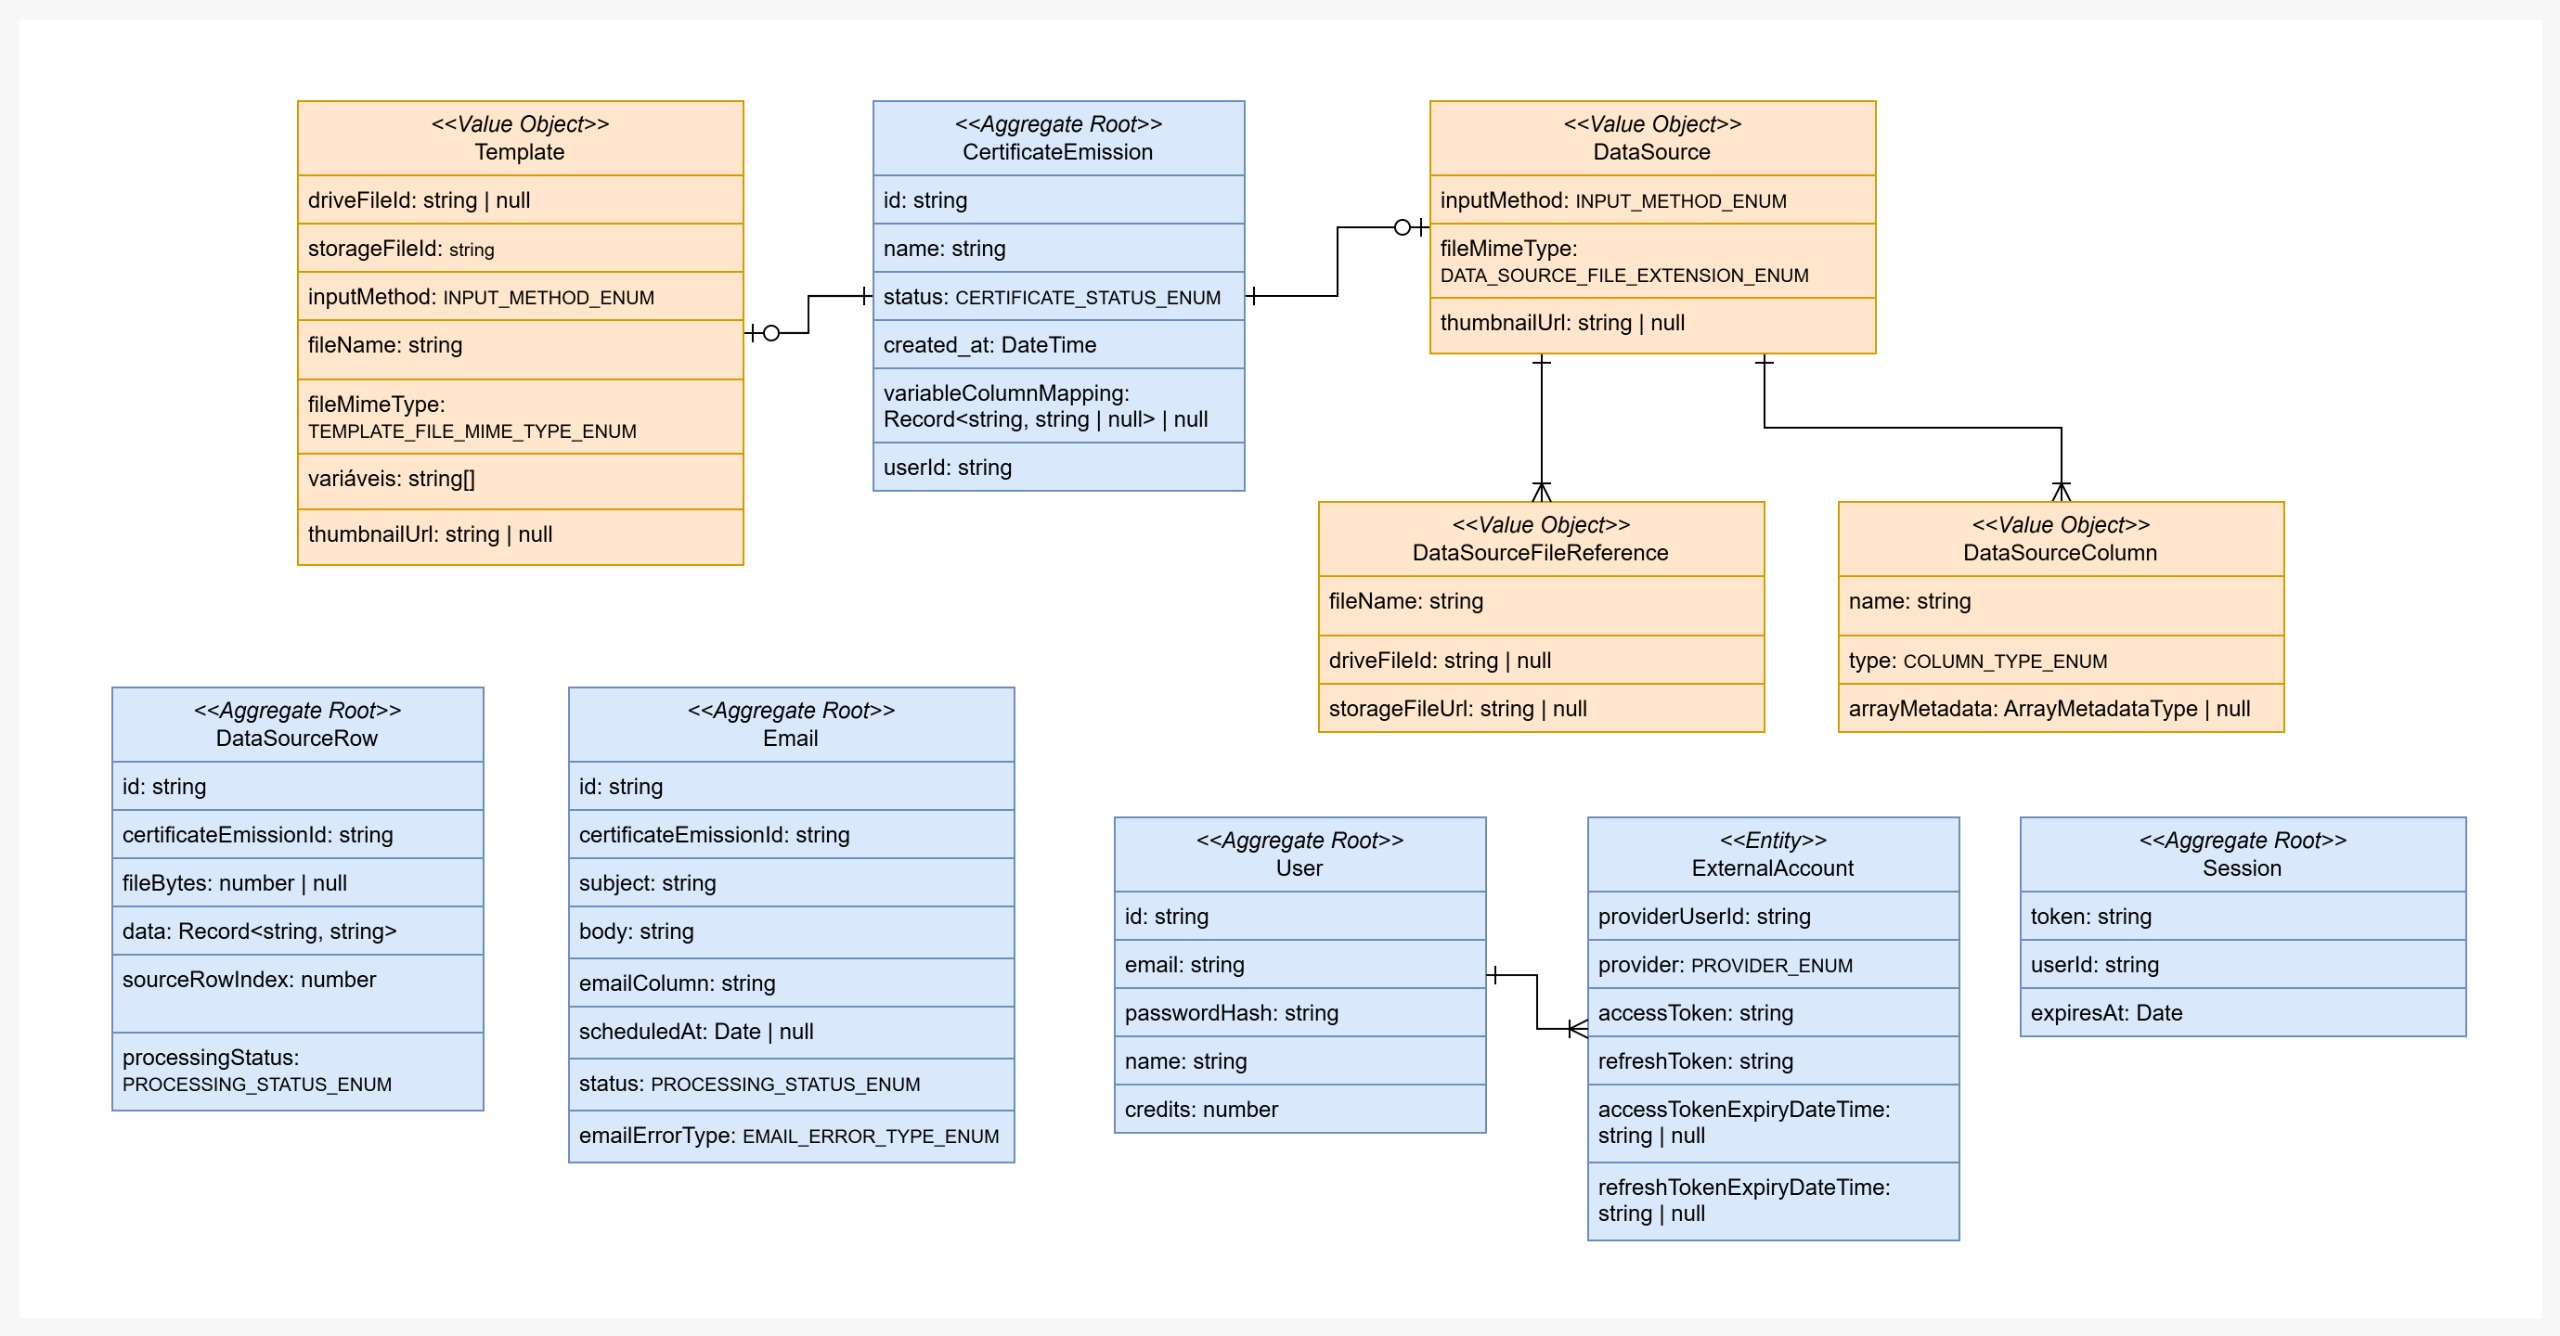
\includegraphics[width=1\textwidth]{context-mapping.png}
    \caption{Diagrama do modelo de domínio.}
    \label{fig:domain_model}
    \fonte{Autoria própria.}
\end{figure}

A separação entre os blocos de construção do domínio (agregados, entidades e objetos de valor) garante que a lógica de negócio permaneça coesa e protegida de detalhes de infraestrutura.

O modelo conta com cinco agregados raiz:

\begin{itemize}
    \item \textbf{CertificateEmission}: elemento central do domínio. Encapsula todo o ciclo de vida de uma emissão de certificados, transitando pelos estados DRAFT, SCHEDULED, GENERATED e EMITTED. Internamente, mantém referências ao template, à fonte de dados e ao mapeamento entre as variáveis Liquid do template e as colunas da planilha.
    
    \item \textbf{User}: centraliza a gestão de autenticação, suportando login por e-mail e senha e integração com provedores externos via OAuth 2.0. Inclui, ainda, o controle de créditos consumidos a cada emissão.
    
    \item \textbf{Email}: representa uma campanha de envio associada a uma emissão, percorrendo os estados PENDING, RUNNING, COMPLETED e FAILED, e acumulando informações sobre erros de entrega, como colunas removidas da fonte de dados ou e-mails inválidos.
    
    \item \textbf{Session}: gerencia o ciclo de vida de uma sessão autenticada, armazenando o token, a data de expiração e o identificador do usuário.
    
    \item \textbf{DataSourceRow}: representa cada linha individual da fonte de dados, carregando o estado de processamento (PENDING, RUNNING, COMPLETED e FAILED) e os valores das células associadas.
\end{itemize}

Além dos agregados, o domínio conta com uma entidade: \textbf{ExternalAccount}, que encapsula as credenciais de uma conta em provedor externo vinculada a um usuário, permitindo que um mesmo usuário possua múltiplos provedores configurados.

Os objetos de valor, imutáveis e definidos exclusivamente por seus atributos, são:

\begin{itemize}
    \item \textbf{Template}: armazena os metadados do arquivo de template (DOCX, PPTX ou referência ao Google Drive) e é responsável pela extração das variáveis Liquid presentes no documento.
    
    \item \textbf{DataSource}: representa a fonte de dados com suas colunas definidas e o arquivo associado.
    
    \item \textbf{DataSourceColumn}: modela o tipo inferido de cada coluna (STRING, NUMBER, BOOLEAN, DATE ou ARRAY).
    
    \item \textbf{DataSourceFile}: guarda a referência ao arquivo no Cloud Storage ou no Google Drive.
    
    \item \textbf{EmailVerificationCode} e \textbf{ResetPasswordCode}: encapsulam tokens de uso único com prazo de expiração para os fluxos de verificação de e-mail e redefinição de senha, respectivamente.
\end{itemize}

Na Figura~\ref{fig:domain_model}, linhas representam relações de composição entre os elementos do modelo. Objetos de valor como \textbf{Template}, \textbf{DataSource} e \textbf{DataSourceFileReference} estão ligados ao agregado \textbf{CertificateEmission} porque fazem parte de sua composição interna, eles não possuem existência independente fora do contexto da emissão. A entidade \textbf{ExternalAccount}, por sua vez, é interna ao agregado \textbf{User}, razão pela qual também aparece conectada a ele. Já os agregados raiz que não possuem linhas entre si, como \textbf{CertificateEmission} e \textbf{DataSourceRow}, ou \textbf{Session} e \textbf{User}, respeitam uma regra importante do DDD: agregados não devem referenciar outros agregados por composição de objeto, mas sim por identidade. Nesses casos, a referência se dá pelo identificador do agregado relacionado (\textit{e.g.}, \texttt{certificateEmissionId} em \textbf{DataSourceRow} e \texttt{userId} em \textbf{Session}), garantindo as fronteiras transacionais e evitando acoplamento entre raízes de agregados distintas. No caso de \textbf{DataSourceRow}, essa separação também foi motivada por razões práticas: como uma emissão pode conter centenas de linhas, incorporá-las diretamente em \textbf{CertificateEmission} tornaria o agregado excessivamente grande, o que viola outra regra de manter agregados pequenos e coesos. Além disso, cada linha possui seu próprio ciclo de vida de processamento, o que reforça a necessidade de fronteiras transacionais próprias.

Ainda sobre decisões de modelagem, a definição do \textbf{DataSourceColumn} impôs um impasse de design: o sistema não pode modificar os dados extraídos do arquivo do usuário, não sendo possível normalizar capitalização, corrigir separadores decimais ou reformatar datas, pois não há como prever de que forma esses valores serão utilizados no template. Diante disso, foi necessário definir critérios explícitos para a inferência de cada tipo. Uma coluna é classificada como booleana se \emph{todos} os seus valores não-vazios pertencerem ao conjunto \{\texttt{true}, \texttt{false}, \texttt{verdadeiro}, \texttt{falso}, \texttt{1}, \texttt{0}\}, sem distinção de capitalização. Assim, uma coluna com os valores \texttt{TRUE}, \texttt{Falso} e \texttt{FALse} é classificada corretamente como booleana. O mesmo princípio se aplica às demais classificações: datas seguem o formato \texttt{DD/MM/AAAA}, com tolerância a inversão de dia e mês, e números contemplam tanto o formato brasileiro (\texttt{1.234,56}) quanto o americano (\texttt{1,234.56}), com detecção automática do separador decimal.

Todos os agregados seguem uma convenção de instanciação: o construtor é usado como porta de entrada que reforça a integridade do domínio. Para a criação no curso de uma operação de negócio, é utilizado o método estático \texttt{create}, que pode fazer validações próprias, instanciar o construtor da própria classe e registrar os eventos de domínio pertinentes, como \texttt{CertificateCreatedDomainEvent}. Para a persistência, cada agregado expõe um método \texttt{serialize()} que converte seu estado interno em um objeto plano, servindo como o ponto de coleta de dados que os repositórios utilizam para construir as operações de escrita no banco de dados.

O domínio conta também com um serviço de domínio: o \texttt{DataSourceDomain\-Service}, que coordena operações que envolvem múltiplos agregados simultaneamente: especificamente a criação de uma fonte de dados e a geração das linhas associadas (\texttt{DataSourceRow}) a partir do conteúdo extraído do arquivo.

\subsection{Autenticação}

O único mecanismo de autenticação no sistema é o \textbf{token opaco}. Independentemente de como o usuário criou sua conta, por e-mail e senha ou por login com Google, toda requisição autenticada é validada por esse token, gerenciado pelo agregado \texttt{Session}. Ao contrário de tokens auto-contidos como o JWT — que carregam um payload decodificável pelo portador —, o token opaco é uma referência aleatória cuja validade só pode ser verificada mediante consulta ao banco de dados. Essa característica torna cada requisição dependente de uma leitura no banco, mas em contrapartida permite a invalidação imediata do token pelo servidor a qualquer momento, algo que tokens auto-contidos não suportam nativamente sem mecanismos adicionais de revogação.

A integração com o \textbf{Google} utiliza o protocolo \textbf{OAuth 2.0}  \cite{rfc6749}, um framework de autorização que permite que o sistema obtenha acesso delegado a recursos externos (no caso, o Google Drive) em nome do usuário, sem que este precise compartilhar suas credenciais diretamente. O fluxo adotado é o \textit{Authorization Code Flow}: o sistema redireciona o usuário ao servidor de autorização do Google, que retorna um código de autorização (\texttt{authorization\_code}) após o consentimento. O backend troca esse código por tokens de acesso e atualização em uma chamada servidor a servidor, mantendo as credenciais fora do alcance do navegador. Esses tokens são representados na entidade \texttt{ExternalAccount} e utilizados exclusivamente para acessar recursos do Google Drive. Eles são independentes da sessão do sistema: se o token de acesso do Google expirar, o usuário permanece autenticado no sistema por meio do seu token opaco, mas precisará reconectar a conta Google para retomar operações que dependam do Drive.

Embora o OAuth 2.0 especifique como obter autorização, ele não define como identificar o usuário. Essa lacuna é preenchida pelo \textbf{OpenID Connect (OIDC)} \cite{openidconnect}, uma camada de identidade construída sobre o OAuth 2.0. O OIDC introduz o \texttt{id\_token}, um JWT assinado pelo provedor de identidade que contém informações verificáveis sobre o usuário autenticado, como identificador único, e-mail e nome. No sistema, o \texttt{id\_token} emitido pelo Google é utilizado para extrair o e-mail do usuário e associá-lo à sua conta local, após o qual uma sessão com token opaco é criada normalmente.

\subsection{Tratamento de Erros}

O tratamento de erros é modelado como parte do domínio. Em vez de propagar instâncias genéricas de \texttt{Error} do JavaScript, o sistema define classes tipadas para cada categoria de falha:

\begin{itemize}
    \item \textbf{AuthenticationError} (HTTP 401): lançado quando a sessão está ausente, inválida ou expirada.
    \item \textbf{ForbiddenError} (HTTP 403): lançado quando o usuário autenticado não possui permissão sobre o recurso solicitado.
    \item \textbf{NotFoundError} (HTTP 404): lançado quando um recurso buscado não existe na base de dados.
    \item \textbf{ConflictError} (HTTP 409): lançado quando há uma tentativa de cadastrar um recurso que já existe, por exemplo registrar um e-mail que já está em uso.
    \item \textbf{ValidationError} (HTTP 422): lançado quando uma operação viola uma regra de negócio, por exemplo tentar iniciar uma geração sem créditos disponíveis.
    \item \textbf{ServiceUnavailableError} (HTTP 503): lançado quando um serviço externo está indisponível.
\end{itemize}

Cada classe carrega um subtipo literal que identifica o cenário específico, como \texttt{`generation-already-in-progress'} ou \texttt{`insufficient-credits'}, permitindo que o cliente diferencie programaticamente as condições de erro sem recorrer a comparação de strings de mensagem.

Na camada de infraestrutura, esse modelo é traduzido para respostas HTTP segundo a RFC 9457 \cite{rfc9457}, que padroniza o formato de respostas de problema em APIs. Cada resposta de erro carrega um objeto JSON com os campos \texttt{type}, \texttt{title} e \texttt{detail}, permitindo que os clientes da API identifiquem e diferenciem programaticamente qualquer condição de falha.

\subsection{Modelagem do Banco de Dados}

A persistência de dados é implementada sobre um banco de dados relacional PostgreSQL, mapeado pelo ORM Prisma \cite{prisma}. O modelo entidade-relacionamento, ilustrado na Figura~\ref{fig:er_diagram}, foi projetado para refletir o modelo de domínio, normalizado até a Terceira Forma Normal.

\begin{figure}[htbp]
    \centering
    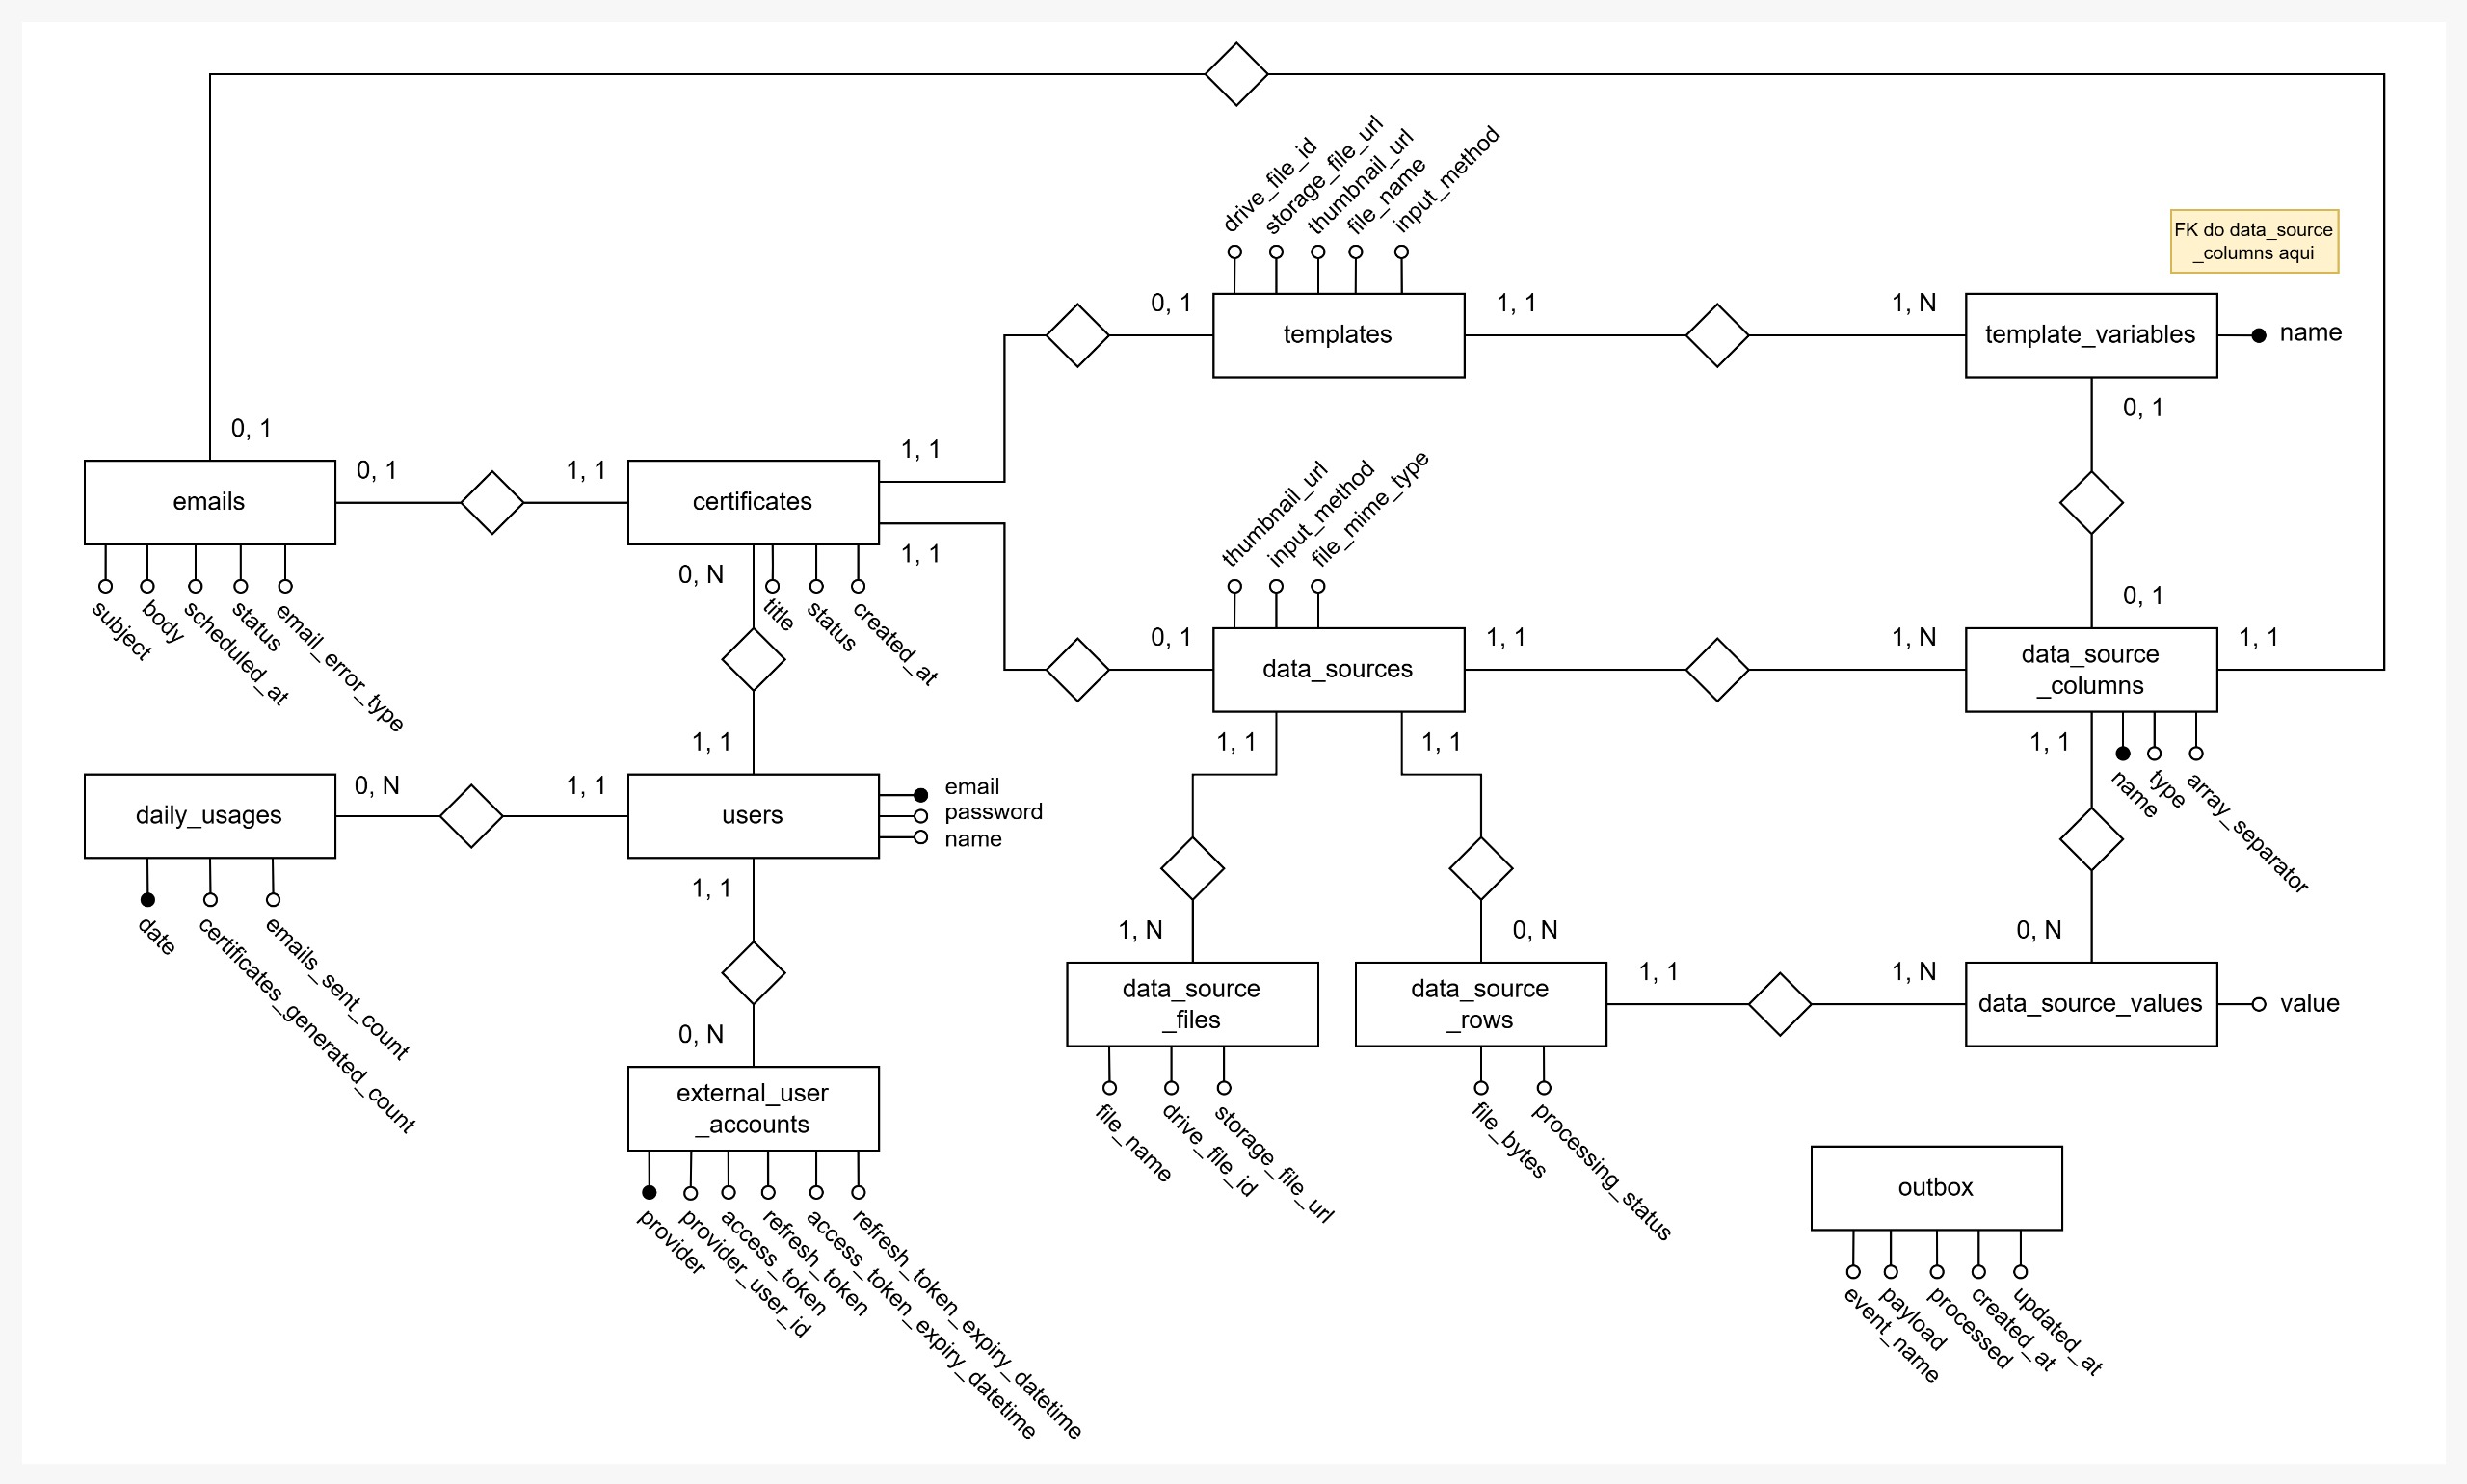
\includegraphics[width=1\textwidth]{db-modeling.png}
    \caption{Diagrama ER do banco de dados.}
    \label{fig:er_diagram}
    \fonte{Autoria própria.}
\end{figure}

A separação entre as tabelas \texttt{DataSourceRow} e \texttt{DataSourceValue} merece destaque como decisão de modelagem relevante. \texttt{DataSourceRow} armazena o estado de processamento de cada linha da fonte de dados (pendente, gerado ou com falha), enquanto \texttt{DataSourceValue} armazena os valores individuais das células em registros separados, com referência à coluna correspondente. Essa estrutura segue a Primeira Forma Normal ao garantir que cada atributo seja atômico e elimina a alternativa de colunas dinâmicas na tabela principal, uma estrutura que, embora mais simples à primeira vista, viola a normalização e torna consultas e atualizações cirúrgicas significativamente mais custosas.

\subsection{Repositórios e Gerenciamento de Transações}

A camada de persistência é implementada por meio de cinco repositórios Prisma: \texttt{PrismaCertificatesRepository}, \texttt{PrismaUsersRepository}, \texttt{PrismaSes\-sionsRepository}, \texttt{PrismaEmailsReposi\-tory} e \texttt{PrismaDataSourceRowsRepository}. Cada repositório é responsável por mapear o estado interno do agregado para o modelo relacional (invocando o método \texttt{serialize()} do agregado para obter o objeto plano que o Prisma utilizará na operação de escrita) e por reconstruir o agregado a partir dos dados retornados pelo banco.

Para operações que exigem consistência transacional entre múltiplos agregados, a camada de aplicação expõe a interface \texttt{ITransactionManager}. Sua implementação concreta, na camada de infraestrutura, utiliza \texttt{AsyncLocalStorage} para propagar o contexto da transação Prisma de forma transparente por toda a pilha de chamadas, sem que os repositórios ou os casos de uso precisem receber o cliente de transação explicitamente como parâmetro.

O gerenciamento de transações é centralizado na classe \texttt{PrismaTransaction\-Manager}, que implementa a interface \texttt{ITransactionManager} definida na camada de aplicação. Quando um caso de uso invoca o método \texttt{run} do gerenciador, este cria uma transação Prisma e armazena o cliente transacional em um \texttt{AsyncLocalStorage}, uma API nativa do Node.js que funciona de maneira análoga a variáveis de contexto de thread em linguagens tradicionais: qualquer código executado dentro da mesma cadeia de chamadas assíncronas pode acessar o valor armazenado, mesmo sem recebê-lo explicitamente como parâmetro. Assim, os repositórios, ao serem chamados dentro desse bloco, detectam automaticamente a presença do cliente transacional no contexto e o utilizam em vez do cliente padrão. Essa abordagem permite que os casos de uso orquestrem operações transacionais complexas, como salvar um certificado e suas linhas de dados atomicamente, mantendo o código de orquestração limpo e livre de preocupações de infraestrutura.

\subsection{Padrões de Projeto: Factory e Strategy}

A extração de conteúdo de diferentes formatos de arquivo é implementada por meio da combinação dos padrões Factory e Strategy. O sistema suporta templates em DOCX e PPTX e fontes de dados em CSV, XLSX e imagem, e a seleção do algoritmo correto para cada formato precisa ser feita em tempo de execução, com base no tipo do arquivo recebido.

O padrão Strategy define uma interface comum para cada família de extratores. Para templates, a interface especifica como extrair as variáveis Liquid presentes no documento. Para fontes de dados, define como ler e estruturar o conteúdo tabular. As implementações concretas (\texttt{DocxContentExtractorStrategy}, \texttt{PptxContent\-ExtractorStrategy}, \texttt{ExcelSpreadsheetContentExtractorStrategy}, \texttt{CSVSpread\-sheetContentExtractorStrategy} e \texttt{ImageContentExtractorStrategy}) encapsulam as bibliotecas específicas de cada formato (\texttt{officeparser}, \texttt{xlsx}, \texttt{csv\-parse}) sem expô-las aos casos de uso.

O padrão Factory materializa a seleção da estratégia correta. \texttt{FileContent\-ExtractorFactory} e \texttt{SpreadsheetContentExtractorFactory} recebem o tipo do arquivo e retornam a implementação adequada. Dessa forma, os casos de uso lidam exclusivamente com a interface do extrator, sem qualquer conhecimento sobre qual biblioteca ou algoritmo está sendo utilizado internamente. A adição de suporte a um novo formato requer apenas a criação de uma nova Strategy e seu registro na Factory correspondente, sem qualquer alteração nos casos de uso existentes, aplicando, na prática, o Princípio do Aberto/Fechado (\textit{Open/Closed Principle}): o sistema está aberto para extensão por meio de novas implementações de Strategy, mas fechado para modificação do código já existente.

\subsection{Fluxos Assíncronos}

\subsubsection{Geração de Certificados}

\begin{figure}[htbp]
    \centering
    \includegraphics[width=1\textwidth]{async-generate-certificates.png}
    \caption{Fluxo assíncrono de geração de certificados.}
    \label{fig:async_generation}
    \fonte{Autoria própria.}
\end{figure}

Quando o usuário aciona a geração, o backend enfileira uma tarefa no Cloud Tasks para cada linha da fonte de dados. A Cloud Function \texttt{generate-pdfs} recebe a requisição HTTP correspondente, contendo os dados da linha e as informações de mapeamento da emissão. Para evitar o custo de múltiplas requisições ao Cloud Storage quando várias linhas de uma mesma emissão são processadas concorrentemente, a função mantém um cache em memória do template, de modo que o arquivo seja baixado do bucket apenas na primeira execução e reutilizado nas demais dentro da mesma instância.

Com o template disponível, entra em ação o algoritmo de substituição de variáveis, cujo funcionamento parte de uma particularidade do formato interno de documentos DOCX e PPTX. Internamente, esses formatos representam o texto como uma hierarquia de elementos XML: parágrafos são compostos por sequências de \textit{runs}, e cada run é uma unidade de texto com formatação uniforme: fonte, tamanho, negrito, cor etc. O problema surge quando uma tag Liquid como \texttt{\{\{ nome\_participante \}\}} é escrita em um editor de texto, pois o processador pode fragmentá-la em múltiplos runs distintos sem que isso seja visível ao usuário. Isso ocorre por marcações internas de autocorreção, alterações pontuais de formatação ou simplesmente pela forma como o editor organiza o XML internamente. O resultado é que a tag \texttt{\{\{ nome\_participante \}\}} pode estar armazenada como três runs separados: \texttt{\{\{}, \texttt{ nome\_participante} e \texttt{\}\}}, tornando a tag irreconhecível por qualquer motor de template.

Para contornar esse problema, o algoritmo percorre cada parágrafo do documento e consolida os runs adjacentes em um único run antes de processar o Liquid, preservando a formatação do primeiro run do grupo. Após a consolidação, o texto completo de cada parágrafo é submetido ao motor Liquid, com os valores da linha sendo substituídos de acordo com o que está definido no template.

Os valores passados ao motor Liquid não são strings simples: são instâncias de classes Python específicas (\texttt{LiquidDate}, subclasse de \texttt{datetime}, e \texttt{LiquidFloat}, subclasse de \texttt{float}) que sobrescrevem o método \texttt{\_\_str\_\_} para retornar a representação original extraída do arquivo. Essa decisão resolve o impasse descrito na modelagem do \texttt{DataSourceColumn}: o sistema não pode modificar os dados do usuário, mas precisa que eles se comportem como tipos nativos para que expressões Liquid funcionem corretamente. Assim, quando o motor Liquid avalia uma expressão condicional como \texttt{\{\% if participou \%\}}, ele opera sobre o valor lógico correto (\texttt{True}/\texttt{False}); quando exibe o valor com \texttt{\{\{ participu \}\}}, retorna a string original tal como estava na planilha, sem qualquer transformação.

Há, contudo, uma limitação decorrente do processamento sequencial do documento: o contexto Liquid é único e acumulado ao longo de toda a renderização, de modo que variáveis definidas com \texttt{\{\% assign \%\}} ou \texttt{\{\% capture \%\}} em um parágrafo estão disponíveis nos parágrafos processados depois. O problema surge quando a ordem de leitura no documento não corresponde à ordem em que as dependências precisam ser resolvidas, ou seja, quando um elemento que consome uma variável (\texttt{\{\{ x \}\}}) aparece antes do elemento que a define (\texttt{\{\% assign x = "valor" \%\}}). Nesse caso, no momento em que o motor Liquid processa a referência, a variável ainda não foi atribuída, e o resultado é uma saída vazia. Templates que declaram variáveis globais após o ponto onde são utilizadas produzirão renderizações incorretas sem emitir erros explícitos.

O documento processado é então enviado ao Google Drive, onde a API do Drive realiza a conversão para PDF nativamente. Após a exportação, o arquivo temporário é removido do Drive e o PDF resultante é armazenado no Cloud Storage em \texttt{users/\{userId\}/certificates/\{emissionId\}/certificate-\{rowId\}.pdf}. Por fim, a Cloud Function notifica o backend por meio de uma requisição PATCH ao endpoint interno \texttt{/api/internals/data-source-rows/\{rowId\}/generations}, atualização o status da linha. O backend, ao processar essa atualização, emite uma mensagem para o mecanismo de SSE, que entrega a atualização de progresso em tempo real ao frontend do usuário.

\subsubsection{Envio de E-mails}

\begin{figure}[htbp]
    \centering
    \includegraphics[width=1\textwidth]{async-send-emails.png}
    \caption{Fluxo assíncrono de envio de e-mails.}
    \label{fig:async_emails}
    \fonte{Autoria própria.}
\end{figure}

Após a conclusão da geração, o usuário pode acionar o envio dos certificados. O backend enfileira uma tarefa no Cloud Tasks com a lista de destinatários e as configurações do e-mail. A Cloud Function \texttt{send-certificate-emails} recebe a requisição e processa os envios concorrentemente, utilizando um pool de cinco threads para baixar os PDFs do Cloud Storage e enviá-los como anexos via Brevo.

A escolha do Brevo como serviço de envio vai além da conveniência de uma API transacional: ela endereça um problema real de entregabilidade. O envio massivo de e-mails com anexos grandes, como certificados em PDF, é frequentemente interceptado por filtros de spam institucionais, que barram mensagens de remetentes não autenticados ou com configurações de domínio inadequadas. Para garantir que os certificados cheguem à caixa de entrada dos destinatários, o sistema configura três padrões de autenticação de e-mail:

\begin{itemize}
    \item \textbf{SPF (Sender Policy Framework)}: um registro DNS que declara explicitamente quais servidores de e-mail estão autorizados a enviar mensagens em nome do domínio do remetente. Ao receber um e-mail, o servidor do destinatário consulta o registro SPF do domínio de origem e rejeita a mensagem caso o servidor remetente não esteja listado. Sem SPF, e-mails enviados pela infraestrutura do Brevo poderiam ser tratados como forjados.
    
    \item \textbf{DKIM (DomainKeys Identified Mail)}: adiciona uma assinatura criptográfica a cada mensagem enviada, gerada com uma chave privada conhecida apenas pelo serviço de envio. O servidor do destinatário verifica a assinatura utilizando a chave pública correspondente, publicada no DNS do domínio. O DKIM garante que o conteúdo do e-mail não foi alterado em trânsito e que a mensagem foi de fato enviada por um remetente autorizado.
    
    \item \textbf{DMARC (Domain-based Message Authentication, Reporting and Conformance)}: uma política publicada no DNS que instrui os servidores receptores sobre como tratar mensagens que falhem na verificação de SPF ou DKIM: se devem ser rejeitadas, movidas para spam ou aceitas. O DMARC também prevê um mecanismo de relatórios, permitindo que o proprietário do domínio monitore tentativas de uso indevido do seu endereço de envio.
\end{itemize}

Juntos, SPF, DKIM e DMARC estabelecem uma cadeia de confiança que valida a identidade do remetente e a integridade da mensagem, reduzindo significativamente a probabilidade de os e-mails serem barrados por filtros corporativos e institucionais. Ao concluir o processamento, a função notifica o backend via PATCH em \texttt{/api/internals/emails/\{emailId\}} com o status final da campanha.

\subsection{Estratégia de Testes}

A suíte de testes automatizados do sistema foi construída seguindo a Pirâmide de Testes, com três níveis distintos: unitários, de integração e de ponta a ponta.

Os testes unitários, executados com o framework Vitest \cite{vitest}, cobrem as camadas de domínio e aplicação em isolamento total, totalizando 578 casos de teste com cobertura de 93,27\% pelo critério todas-arestas. As suítes de domínio verificam os invariantes de negócio, as transições de estado e o comportamento dos factory methods. Os testes de casos de uso utilizam os dublês de testes necessários para cada caso sem nenhuma dependência de framework ou serviço de nuvem.

Os testes de integração também utilizam o Vitest, mas são executados contra um banco de dados PostgreSQL real, instanciado sob demanda com o TestContainers \cite{testcontainers}, uma biblioteca que permite provisionar e gerenciar containers Docker diretamente do código de teste, garantindo um ambiente reproduzível sem configuração manual de infraestrutura. Antes da execução da suíte, o TestContainers inicializa o container e aplica as migrações do banco de dados; ao término, o container é destruído. Para cada teste individualmente, todas as tabelas são truncadas, garantindo que o estado inicial seja sempre previsível e que os testes sejam completamente independentes entre si. A suíte conta com 65 casos de teste de integração, verificando que os repositórios Prisma mapeiam corretamente os agregados para o modelo relacional e que as transações se comportam conforme especificado.

No topo da pirâmide, os testes de ponta a ponta são implementados com o Playwright \cite{playwright}, um framework de automação de navegadores desenvolvido pela Microsoft que permite controlar instâncias reais de Chromium, Firefox e WebKit programaticamente, simulando com fidelidade as interações de um usuário real. O banco de dados também é provisionado com TestContainers, seguindo a mesma abordagem dos testes de integração; para cada teste, o estado da aplicação (usuários, sessões e dados gerados) é limpo para garantir a independência entre os cenários. Os 8 casos de teste E2E cobrem os fluxos críticos do sistema e são executados em paralelo nos quatro ambientes de navegação (Chromium, Firefox, WebKit e Microsoft Edge), garantindo compatibilidade entre os principais motores de renderização.

Além dos três níveis da pirâmide, a qualidade dos testes unitários foi avaliada com testes de mutação executados pelo Stryker \cite{stryker}, atingindo um score de mutação de 82\% na camada de domínio, onde residem as regras de negócio críticas do sistema.

\subsection{Integração e Entrega Contínuas}

A suíte de testes é integrada ao workflow de CI/CD como pré-condição para qualquer implantação, operando como mecanismo de teste de regressão: a cada modificação submetida à branch principal, os três níveis da pirâmide são reexecutados, garantindo que nenhuma alteração chegue ao ambiente de produção sem ter sido validada e sem ter introduzido quebras em funcionalidades previamente estáveis. O GitHub Actions é a plataforma de automação de fluxos de trabalho utilizada. No sistema, a esteira de CI/CD é implementada em um único workflow composto por quatro jobs sequenciais (\texttt{test}, \texttt{terraform-plan}, \texttt{terraform-apply} e \texttt{deploy}), conforme ilustrado na Figura~\ref{fig:cicd}.

\begin{figure}[htbp]
    \centering
    \includegraphics[width=1\textwidth]{ci-cd.png}
    \caption{Esteira de CI/CD do sistema no GitHub Actions.}
    \label{fig:cicd}
    \fonte{Autoria própria.}
\end{figure}

O job \textbf{test} instala as dependências da aplicação e executa a suíte completa de testes automatizados. Somente após a aprovação desse job os demais são iniciados. A autenticação com o Google Cloud é realizada via Workload Identity Federation, permitindo obter credenciais temporárias de curta duração diretamente do GCP.

O job \textbf{terraform-plan} inicializa o Terraform com um backend de estado remoto armazenado em um bucket do Cloud Storage. Com o estado carregado, o job executa o planejamento e persiste o plano gerado como artefato. O job \textbf{terraform-apply} baixa os artefatos produzidos e aplica o plano de infraestrutura.

O job \textbf{deploy} constrói a imagem Docker da aplicação Next.js em múltiplos estágios para resultar em uma imagem enxuta no modo standalone. A imagem é publicada no Artifact Registry com a tag correspondente ao hash do commit. Antes da substituição da imagem em produção, as migrations Prisma são executadas contra o banco de dados. Por fim, o Cloud Run é atualizado para servir a nova revisão.

A nomenclatura dos recursos Terraform com sufixo de branch permite que o sistema opere em ambientes completamente isolados por branch, possibilitando validar o sistema em condições idênticas às de produção antes de qualquer fusão ao branch principal.

\section{Avaliação}\label{sec:avaliacao}

Esta seção apresenta um estudo piloto conduzido para validar a solução desenvolvida. A análise combina abordagem quantitativa, por meio de estatística descritiva das escalas Likert, e qualitativa, por meio de análise temática das respostas abertas.

\subsection{Coleta de Feedback}

Concluída a implementação do sistema, a versão final foi submetida a um processo de validação empírica por meio de um estudo piloto com 12 participantes pertencentes ao público-alvo da ferramenta: pessoas que organizam eventos acadêmicos e precisam emitir certificados.

Os participantes foram divididos em dois perfis. Dois usuários possuíam um caso real de emissão de certificados e utilizaram seus próprios arquivos e dados durante o experimento. Os demais operaram em modo simulado, utilizando materiais de exemplo disponibilizados e seguindo tarefas sugeridas.

O processo foi estruturado em dois momentos. Antes do uso, os participantes preencheram um formulário de consentimento e perfil, que registrou nome, área de atuação, facilidade autodeclarada com tecnologia e se possuíam um caso real de emissão de certificados. A Tabela~\ref{tab:perfil-participantes} sintetiza o perfil dos participantes com base nessas informações, preservando o anonimato de cada um.

\begin{table}[htbp]
    \centering
    \caption{Perfil dos participantes do estudo piloto.}
    \label{tab:perfil-participantes}
    \begin{tabular}{|C{1.5cm}|C{3.5cm}|C{2.5cm}|C{3.5cm}|}
        \hline
        \textbf{Part.} & \textbf{Área de atuação} & \textbf{Facilidade com tecnologia (1--5)} & \textbf{Caso real} \\
        \hline
        P1  & Tecnologia          & 5 & Não \\
        \hline
        P2  & Computação (docente) & 5 & Não \\
        \hline
        P3  & Computação (docente) & 4 & Sim \\
        \hline
        P4  & Computação (docente) & 4 & Sim \\
        \hline
        P5  & Computação (discente) & 4 & Não \\
        \hline
        P6  & Computação (discente) & 5 & Não \\
        \hline
        P7  & Computação (discente) & 5 & Não \\
        \hline
        P8  & Computação (discente) & 5 & Não \\
        \hline
        P9  & Computação (discente) & 5 & Não \\
        \hline
        P10 & Tecnologia           & 4 & Não \\
        \hline
        P11 & Computação (discente) & 5 & Não \\
        \hline
        P12 & Computação (discente) & 5 & Não \\
        \hline
    \end{tabular}

    \fonte{Elaboração própria.}
\end{table}

A maioria dos participantes era composta por discentes de graduação, com participação de docentes e profissionais da área de tecnologia. A facilidade autodeclarada com sistemas web e novas tecnologias concentrou-se nas faixas 4 e 5, indicando um público predominantemente experiente com tecnologia. Após a experiência, responderam a um formulário de avaliação com perguntas em escala Likert \cite{likert1932technique} de 1 a 5 e com perguntas abertas, conforme listado na Tabela~\ref{tab:perguntas-avaliacao}.

\begin{table}[htbp]
    \centering
    \caption{Perguntas do formulário de avaliação pós-uso.}
    \label{tab:perguntas-avaliacao}
    \begin{tabular}{|C{1cm}|C{2.5cm}|C{8.5cm}|}
        \hline
        \textbf{ID} & \textbf{Tipo} & \textbf{Pergunta} \\
        \hline
        Q1  & Likert (1--5) & Quão fácil foi fazer todo o fluxo de emissão de certificados? \\
        \hline
        Q2  & Likert (1--5) & Quanto esforço cognitivo foi necessário para a emissão de certificados? (1 = Muito esforço / 5 = Nenhum esforço) \\
        \hline
        Q3  & Fechada (S/N) & Você encontrou algum problema técnico ou erro durante o uso? \\
        \hline
        Q4  & Aberta & Se sim, descreva o problema técnico ou erro encontrado. \\
        \hline
        Q5  & Fechada (S/N) & A ferramenta permitiu que você customizasse o certificado conforme esperado? \\
        \hline
        Q6  & Aberta & Descreva como foi a customização do certificado e se atendeu às suas necessidades. \\
        \hline
        Q7  & Aberta & Quais funcionalidades mais se destacaram na sua opinião? \\
        \hline
        Q8  & Fechada (S/N) & Sentiu falta de alguma funcionalidade? \\
        \hline
        Q9  & Aberta & Se sim, descreva a funcionalidade que sentiu falta. \\
        \hline
        Q10 & Likert (1--5) & Quanto esforço você economizou ao usar o sistema para gerar certificados? \\
        \hline
        Q11 & Likert (1--5) & Quanto o sistema pareceu estável durante o uso? (1 = Propenso a erros / 5 = Muito consistente) \\
        \hline
        Q12 & Likert (1--5) & Quanto você se sentiu seguro ao usar o sistema? \\
        \hline
        Q13 & Likert (1--5) & Qual a probabilidade de você utilizar este sistema em uma futura necessidade de emissão de certificados? \\
        \hline
        Q14 & Likert (1--5) & Qual a probabilidade de você recomendar este sistema para outra pessoa que precisa gerar certificados? \\
        \hline
        Q15 & Aberta & Você possui algum comentário adicional sobre o sistema ou sobre o experimento? \\
        \hline
    \end{tabular}

    \fonte{Elaboração própria.}
\end{table}

\subsection{Resultados Quantitativos}

A Figura~\ref{fig:likert-medias} apresenta a distribuição das respostas e as médias da escala Likert por dimensão avaliada, considerando os 12 participantes que concluíram o formulário pós-uso. Visualmente, a forte concentração das barras à direita do eixo central (0\%) evidencia um alto grau de satisfação e percepções positivas em relação ao sistema.

% Cores do Likert
\definecolor{likert1}{RGB}{202,0,32}
\definecolor{likert2}{RGB}{244,165,130}
\definecolor{likert3}{RGB}{186,186,186}
\definecolor{likert4}{RGB}{146,197,222}
\definecolor{likert5}{RGB}{5,113,176}


\begin{figure}[htbp]
\centering
\begin{tikzpicture}
\begin{axis}[
    xbar stacked,
    xmin=-35, xmax=115, % Espaço extra no xmax para caber a média
    width=11cm, height=7.5cm,
    bar width=0.45cm,
    ytick=data,
    yticklabels={
        Facilidade do fluxo,
        Esforço cognitivo,
        Esforço economizado,
        Estabilidade percebida,
        Segurança percebida,
        Prob.\ de reuso,
        Prob.\ de recomendação
    },
    yticklabel style={font=\small, align=right, text width=4.5cm},
    xlabel={Proporção de respostas (\%)},
    xtick={-25,0,25,50,75,100},
    % É padrão em gráficos Likert divergentes usar valores absolutos nos dois lados
    xticklabels={25, 0, 25, 50, 75, 100}, 
    enlarge y limits=0.12,
    legend style={
        at={(0.5,1.05)},
        anchor=south,
        legend columns=5,
        font=\scriptsize,
        column sep=1ex,
    },
    legend cell align=left,
]

% 1. LEGENDAS MANUAIS (Para não depender da ordem dos gráficos abaixo)
\addlegendimage{fill=likert1, area legend}
\addlegendimage{fill=likert2, area legend}
\addlegendimage{fill=likert3, area legend}
\addlegendimage{fill=likert4, area legend}
\addlegendimage{fill=likert5, area legend}
\legend{1, 2, 3, 4, 5}

% 2. BARRAS NEGATIVAS (Do centro para a esquerda: Metade do 3 -> 2 -> 1)
\addplot[fill=likert3, forget plot] coordinates {(0,0) (-16.7,1) (-4.2,2) (-4.2,3) (-5.0,4) (0,5) (0,6)};
\addplot[fill=likert2, forget plot] coordinates {(-8.3,0) (0,1) (0,2) (0,3) (-10.0,4) (0,5) (0,6)};
\addplot[fill=likert1, forget plot] coordinates {(0,0) (0,1) (0,2) (0,3) (0,4) (0,5) (0,6)};

% 3. BARRAS POSITIVAS (Do centro para a direita: Metade do 3 -> 4 -> 5)
\addplot[fill=likert3, forget plot] coordinates {(0,0) (16.7,1) (4.2,2) (4.2,3) (5.0,4) (0,5) (0,6)};
\addplot[fill=likert4, forget plot] coordinates {(50.0,0) (33.3,1) (0,2) (16.7,3) (30.0,4) (16.7,5) (16.7,6)};
\addplot[fill=likert5, forget plot] coordinates {(41.7,0) (33.3,1) (91.7,2) (75.0,3) (50.0,4) (83.3,5) (83.3,6)};

% 4. PLOTAGEM DAS MÉDIAS
% Usamos as coordenadas absolutas calculadas pela soma das barras positivas
\node[anchor=west, font=\scriptsize\bfseries] at (axis cs: 91.7, 0) { 4,25};
\node[anchor=west, font=\scriptsize\bfseries] at (axis cs: 83.3, 1) { 4,00};
\node[anchor=west, font=\scriptsize\bfseries] at (axis cs: 95.9, 2) { 4,83};
\node[anchor=west, font=\scriptsize\bfseries] at (axis cs: 95.9, 3) { 4,67};
\node[anchor=west, font=\scriptsize\bfseries] at (axis cs: 85.0, 4) { 4,20};
\node[anchor=west, font=\scriptsize\bfseries] at (axis cs: 100.0, 5) { 4,83};
\node[anchor=west, font=\scriptsize\bfseries] at (axis cs: 100.0, 6) { 4,83};

\end{axis}
\end{tikzpicture}
\caption{Gráfico divergente das respostas na escala Likert por dimensão avaliada, com médias indicadas ao final de cada barra.}
\label{fig:likert-medias}

\fonte{Elaboração própria.}

\end{figure}

Nenhum dos participantes relatou erros técnicos durante o uso. As dimensões de probabilidade de reuso, de recomendação e de esforço economizado obtiveram as maiores médias (4,8 de 5), indicando forte intenção de uso futuro e aprovação da solução, e confirmando que o sistema cumpre seu objetivo central de reduzir o trabalho manual associado à emissão de certificados.

\subsection{Análise Qualitativa}

\subsubsection{Pontos Positivos}

A centralização de todo o fluxo em uma única plataforma foi o ponto mais recorrente nas avaliações positivas. Participantes destacaram a eliminação da necessidade de alternar entre ferramentas distintas para gerar e distribuir os certificados. A integração com o Google Drive, que permite importar templates e fontes de dados diretamente do drive do usuário, foi citada como um diferencial relevante. A funcionalidade de extração automática de dados da fonte, incluindo a leitura de imagens com auxílio de inteligência artificial, e o envio automático de e-mails com os certificados anexados foram os recursos mais elogiados. O mapeamento entre variáveis Liquid e colunas da planilha também recebeu menções positivas pela clareza conceitual da operação.

Do ponto de vista de usabilidade, participantes comentaram que a interface apresenta as seções progressivamente, sem sobrecarregar o usuário com informações de uma só vez, o que contribuiu para uma experiência percebida como leve e guiada.

\subsubsection{Pontos de Melhoria}

A crítica mais recorrente foi a ausência de instruções mais didáticas. Múltiplos participantes, incluindo os dois usuários de casos reais, relataram dificuldades iniciais para compreender o fluxo completo, especialmente a relação entre o template Liquid, a fonte de dados e o mapeamento de variáveis. Sugestões incluíram a adição de um vídeo demonstrativo, um tutorial em texto na área de ajuda e mensagens contextuais mais claras durante o fluxo.

A impossibilidade de editar células da fonte de dados diretamente pelo sistema foi apontada por uma participante do caso real: atualmente, qualquer correção exige que o usuário baixe o arquivo, edite externamente e o reimporte. Uma participante do caso real levantou também a ausência de controle sobre emissões já concluídas: após o envio, não é possível editar o template, corrigir endereços de e-mail ou excluir registros do painel. Outros participantes sentiram falta de um editor ou gerador de templates integrado à plataforma, eliminando a necessidade de criar o documento em ferramentas externas como Word ou Google Slides.

Um participante relatou que as permissões solicitadas pelo sistema no momento do login com Google pareceram intrusivas. Essas permissões de acesso ao Google Drive são necessárias para habilitar a importação de templates e fontes de dados diretamente do drive do usuário, dispensando o download e o reupload manual dos arquivos.

Uma participante mencionou lentidão na resposta do sistema. Esse comportamento está associado às restrições de infraestrutura do ambiente acadêmico de avaliação: o serviço foi implantado com configuração mínima de recursos computacionais no Cloud Run e utiliza um banco de dados PostgreSQL gratuito no Supabase, que possui capacidade reduzida também. Essa limitação é inerente ao contexto de prototipagem e não reflete o desempenho esperado em uma implantação com recursos adequados à carga de uso.

Vale destacar que, mesmo entre os participantes que relataram maior dificuldade de uso, a percepção de valor permaneceu alta: um dos casos reais apresentou a menor nota de facilidade de todo o grupo (2/5), mas atribuiu nota máxima para esforço economizado e intenção de reuso (5/5), evidenciando que o valor entregue pelo sistema superou o atrito da curva de aprendizado inicial.

\subsection{Síntese}

Em conjunto, os resultados quantitativos e qualitativos convergem para uma avaliação positiva da solução. A alta intenção de reuso e recomendação indica que o sistema entrega valor percebido suficiente para justificar o custo de adoção. O principal gap identificado não é de funcionalidade, mas de \textit{onboarding}: a ausência de um tutorial ou guia contextual mais claro eleva desnecessariamente a carga cognitiva inicial, sobretudo para usuários sem familiaridade prévia com os conceitos de templates e mapeamento de variáveis. As demais lacunas apontadas (edição inline da fonte de dados, gerenciamento pós-emissão com exclusão de dados, gerador de templates integrado e assinatura digital) são consistentes com as direções de trabalho futuro descritas na seção seguinte.

\section{Conclusão}\label{sec:conclusao}

O Certifica foi concebido com dois objetivos complementares: resolver um problema operacional real, a ineficiência na geração e emissão em lote de certificados, e construir um software tecnicamente consistente desde a concepção. Ambos os objetivos foram atendidos.

Do ponto de vista técnico, o sistema foi construído sobre os princípios da Clean Architecture e do Domain-Driven Design, com o domínio de negócio completamente isolado de detalhes de infraestrutura. A suíte de testes automatizados cobre os três níveis da pirâmide, com testes unitários atingindo mais de 90\% de cobertura pelo critério todas-arestas e mais de 80\% de score de mutação na camada de domínio, complementados por testes de integração e casos de ponta a ponta executados em quatro navegadores. Toda a infraestrutura é provisionada como código via Terraform, e o ciclo de entrega contínua é totalmente automatizado pelo GitHub Actions, garantindo que o sistema esteja sempre implantado e testado a cada modificação.

Do ponto de vista da validação com usuários, os resultados do estudo piloto confirmaram que a solução entrega valor real ao público-alvo. Nenhum participante relatou erros técnicos durante o uso, e as dimensões de intenção de reuso, de recomendação e de esforço economizado obtiveram médias de 4,8 de 5. A percepção de valor permaneceu alta mesmo entre os participantes que relataram maior dificuldade inicial, evidenciando que o principal atrito não é de funcionalidade, mas de \textit{onboarding}: a ausência de instruções mais didáticas para guiar usuários menos familiarizados com os conceitos de templates e mapeamento de variáveis.

Apesar dos bons resultados observados, algumas direções de evolução foram identificadas ao longo do desenvolvimento. Essas direções estão descritas a seguir.

\vspace{3mm}\noindent\textbf{Gestão de Certificados Gerados.}
%
O fluxo atual de geração trata o lote como uma unidade indivisível: se um certificado apresentar um erro de dados, o usuário precisa corrigir o arquivo externo, reimportar a fonte de dados e reiniciar a geração. Três melhorias endereçariam essa limitação diretamente.

A primeira é a \textbf{edição de dados da fonte} diretamente pela interface: permitir que o usuário altere o valor de células individuais sem precisar baixar, editar e reenviar a planilha. A segunda é a \textbf{regeração individual}: uma vez identificado o certificado com problema, poder regerá-lo isoladamente sem refazer o lote inteiro. A terceira é a \textbf{geração de certificado de amostra}: antes de iniciar o processamento completo, gerar um único PDF de prévia com a primeira linha ou com dados informados pelo usuário, permitindo validar o resultado do template antes de comprometer os créditos do lote.

\vspace{3mm}\noindent\textbf{Autenticidade e Verificação.}
%
À medida que certificados digitais substituem documentos físicos, a capacidade de verificar sua autenticidade torna-se essencial. Duas extensões cobrem esse cenário. A \textbf{validação pública} associaria a cada certificado gerado uma URL única, impressa no documento como QR code, que qualquer pessoa poderia acessar para confirmar a autenticidade e os dados da emissão, funcionalidade especialmente útil em contextos de RH e processos seletivos. Complementarmente, a \textbf{assinatura digital} adicionaria uma assinatura criptográfica ao PDF, garantindo que o conteúdo não foi adulterado após a emissão e tornando o documento verificável mesmo sem acesso ao sistema.

\vspace{3mm}\noindent\textbf{Integrações.}
%
O sistema atualmente opera de forma fechada: não há mecanismo para que ferramentas externas saibam quando uma geração ou envio foi concluído. A disponibilização de \textbf{webhooks configuráveis} permitiria que o usuário cadastrasse URLs acionadas automaticamente ao término de eventos específicos, como a conclusão de um lote ou o envio de e-mails, integrando o Certifica a plataformas externas sem necessidade de polling ou intervenção manual.

\vspace{3mm}\noindent\textbf{Colaboração.}
%
O modelo atual é estritamente individual: cada emissão pertence a um único usuário. A introdução de \textbf{espaços de trabalho multi-usuário} permitiria que equipes responsáveis por eventos colaborassem na mesma emissão com papéis distintos, como organizador e revisor, eliminando a necessidade de compartilhar credenciais ou exportar dados entre contas.

\vspace{3mm}\noindent\textbf{Geração de Templates com Inteligência Artificial.}
%
Atualmente, o usuário precisa criar o template em ferramentas externas, como Google Docs, Slides ou Word, antes de importá-lo. Integrar um \textbf{editor de templates assistido por IA} diretamente na plataforma eliminaria essa dependência: o usuário descreveria o layout desejado e a IA geraria o documento, já com as variáveis Liquid posicionadas e prontas para mapeamento, reduzindo significativamente a barreira de entrada para novos usuários.

\section{Uso de Inteligência Artificial Generativa}\label{sec:ia-generativa}

Este trabalho contou com o auxílio de ferramentas de inteligência artificial generativa em diferentes etapas do processo. O ChatGPT, o Gemini e o Claude foram utilizados de forma alternada ao longo do projeto, apoiando tarefas como escrita e revisão de código, revisão textual e correção ortográfica do artigo. Na fase final do desenvolvimento, o Claude Code passou a ser utilizado também como agente de codificação, automatizando tarefas de implementação de forma mais autônoma. Todo o conteúdo gerado ou sugerido por essas ferramentas foi revisado, validado e adaptado pelo autor, que assume integral responsabilidade pelo resultado final do trabalho.


\newpage
\bibliography{references}

\begin{appendices}

\newpage
\chapter{Lista de ilustrações}
\vspace{-35pt}
\renewcommand{\listfigurename}{}
\listoffigures

\end{appendices}

\newpage
\chapter*{Agradecimentos}
\addcontentsline{toc}{chapter}{Agradecimentos}

Agradeço, em primeiro lugar, ao meu orientador, João Felipe Pimentel, pelo grande suporte desde o início do trabalho. Ele teve uma ótima condução do projeto, me ajudou a gerenciar e enriquecer o escopo e me deu total liberdade para desenvolver. Mesmo após sua saída formal da UFF, continuou acompanhando o projeto de perto e contribuindo com feedbacks valiosos, o que foi fundamental para que eu atingisse todos os objetivos desse trabalho.

À minha coorientadora, Vânia de Oliveira Neves, que aceitou o convite para somar forças na reta final, garantindo a continuidade e a solidez necessárias para a conclusão desse projeto diante da saída do João.

À minha mãe, pelo apoio incondicional e incentivo desde o meu primeiro dia na universidade, sendo a base que me permitiu fazer esse curso com segurança e determinação.

Aos meus amigos, que tornaram a rotina acadêmica mais leve e me apoiaram de inúmeras formas ao longo de toda a graduação. Um agradecimento especial à Mayara e à Bruna, pelo companheirismo, pelas discussões e pelo suporte nos momentos mais difíceis do curso.

Por fim, encerro com a satisfação de ter desenvolvido um projeto que reflete exatamente o que busco como profissional: construir soluções com qualidade e alinhadas ao negócio. Foi uma enorme satisfação poder experimentar e aplicar todo o conhecimento adquirido tanto na faculdade quanto no mercado. Os frutos colhidos, desde o amadurecimento técnico até a visão estratégica de engenharia, superaram minhas expectativas.


\end{document}